\documentclass{book}

\usepackage{float}
\usepackage{amsmath}
\usepackage[german]{babel}
\usepackage{amssymb}
\usepackage{amsxtra}
\usepackage[dvips]{epsfig,psfrag}
\usepackage{listings}
\usepackage{enumitem}

\newcommand{\refchapter}[1]{Kapitel~\ref{#1}}
\newcommand{\refsec}[1]{Sektion~\ref{#1}}
\newcommand{\refeqn}[1]{Gleichung~(\ref{#1})}
\newcommand{\reffig}[1]{Abbildung~\ref{#1}}

\title{\bf CES Softwareentwicklungspraktikum \\
{\small Analyse- und Entwurfsdokument} \vspace{1cm}\\
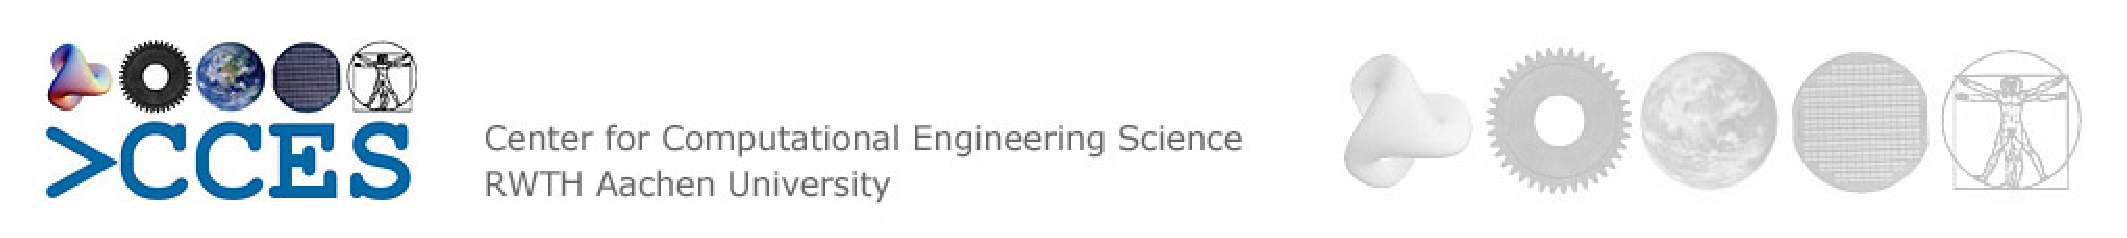
\epsfig{file=figures/cces_logo.eps,width=\textwidth}
}


\author{Stefan Jeske, Daniel Partida, Tom Witter und Chun-Kan Chow}
\date{Matr.-Nr. 334033, 335179, 333265, 333715 \\
email: {\tt [stefan.jeske|daniel.partida|tom.witter|chun-kan.chow]\\
@rwth-aachen.de} 
}

\begin{document}

\lstloadlanguages{[ISO]C++}
\lstset{basicstyle=\small, numbers=left, numberstyle=\footnotesize,
  stepnumber=1, numbersep=5pt, breaklines=true, escapeinside={/*@}{@*/}}


\pagestyle{headings}

\maketitle

\tableofcontents

\chapter{Vorwort}
\label{ch:1}

\section{Aufgabenstellung und Struktur des Dokuments}
\label{sec:1.1}

Sehr geehrte Damen und Herren, \\
\hfill \\
\noindent Bitte entwerfen und implementieren sie eine Applikation, die die Interpolation von Werten
zwischen festgelegten Punkten in einer X-Y-Ebene erlaubt. Die Interpolation soll genutzt
werden, um die Punkte graphisch mit einer Linie zu verbinden.\\
Die Interpolationsroutine soll f\"ur m Kontrollpunkte die X- und Y-Koordinaten von n St\"utzstellen berechnen, die \"aquidistant (Abstand dx) im Intervall [xmin; xmax] verteilt liegen. \\
\noindent Ausschlaggebend f\"ur eine gute Integration der Software in unseren Arbeitsprozess ist, dass
mithilfe einer graphischen Benutzerschnittstelle die Randbedingungen und die Interpolationsart eingestellt werden k\"onnen.\\
\noindent Weiterhin soll eine Visualisierung der resultierenden Interpolation auf der Benutzeroberfl\"ache m\"oglich sein. \\ \\
\noindent Wir freuen uns auf eine Zusammenarbeit. \\ 
\clearpage

\section{Projektmanagement}
\label{sec:1.2}

Tom Witter:
\begin{itemize}
\item Benutzeranforderungen
\item Implementation InterpolationControl
\end{itemize}
Stefan Jeske:
\begin{itemize}
\item Benutzerdokumentation
\item Implementation MainWindow, User Interface
\end{itemize}
Daniel Partida:
\begin{itemize}
\item Aufgabenstellung und Struktur des Dokuments
\item Implementation MainWindow
\end{itemize}
Chun-Kan Chow:
\begin{itemize}
\item Entwicklerdokumentation
\item Implementation Interpolationsarten (CubicSpline, PolynomialInterpolation)
\end{itemize}
Alle:
\begin{itemize}
\item Aktivit\"atsdiagramme
\item UC Beschreibungen
\item funktionale und nicht funktionale Anforderungen
\item Begriffsanalyse
\item Sequenzdiagramme
\item Klassendiagramm
\item Check
\end{itemize}


\section{Lob und Kritik}
\label{sec:1.3}

Danke Naumann f\"ur die Organisation des Projektes und die gewonnene Praxiserfahrung. ;-)


\chapter{Analyse}
\label{ch:2}

\section{Anforderungsanalyse}
\label{sec:2.1}

\subsection{Benutzeranforderungen}
Die Applikation erm\"oglicht es dem Benutzer, verschiedene Punkte in ein Koordinatensystem einzutragen und diese durch Interpolation graphisch zu verbinden.\\
\\
Die Applikation gibt dabei zun\"achst ein 100x50 Koordinatensystem auf der X-Y-Ebene vor.\\
Auf der Benutzeroberfl\"ache kann der Benutzer die Gr\"o\ss e des Koordinatensystems, bzw. den Definitionsbereich ver\"andern.\\
Mit der linken Maustaste kann der Benutzer Punkte im abgebildeten Koordinatensystem auf der Zeichenfl\"ache einzeichnen und mit einem rechten Mausklick auf einen Punkt kann der Benutzer diesen l\"oschen.
Ist mehr als ein Punkt in dem angeklickten L\"oschradius, so l\"oscht die Applikation den Punkt mit dem kleinsten x-Wert.\\
Sind mindestens zwei Punkte eingezeichnet, nachdem ein Punkt hinzugef\"ugt oder gel\"oscht wurde, dann startet die Applikation automatisch die Interpolation und verbindet die eingezeichneten Punkte auf der Zeichenfl\"ache mithilfe der gew\"ahlten Interpolationsmethode.\\
Der Benutzer kann auf einer Auswahlbox auf der Benutzeroberfl\"ache zwischen einer Interpolation durch ein Polynom (Grad m-1 bei m zu Interpolierenden Punkten), oder durch lineare oder kubische Splines w\"ahlen.\\
Nach dem Start des Programmes oder nach dem Zur\"ucksetzen ist die Interpolationsart standardm\"a\ss ig auf lineare Splines eingestellt.\\
Der Benutzer kann zu jeder Zeit  mit dem Button "'Reset"  das leere 100x50 Koordinatensystem mit den Standardeinstellungen wiederherstellen oder mit dem Button "'Beenden" das Programm beenden. \\
\\
\subsection{Anwendungsfallanalyse}

\textbf{Anwendungsfalldiagramm:}

\begin{figure}[H]
\centering
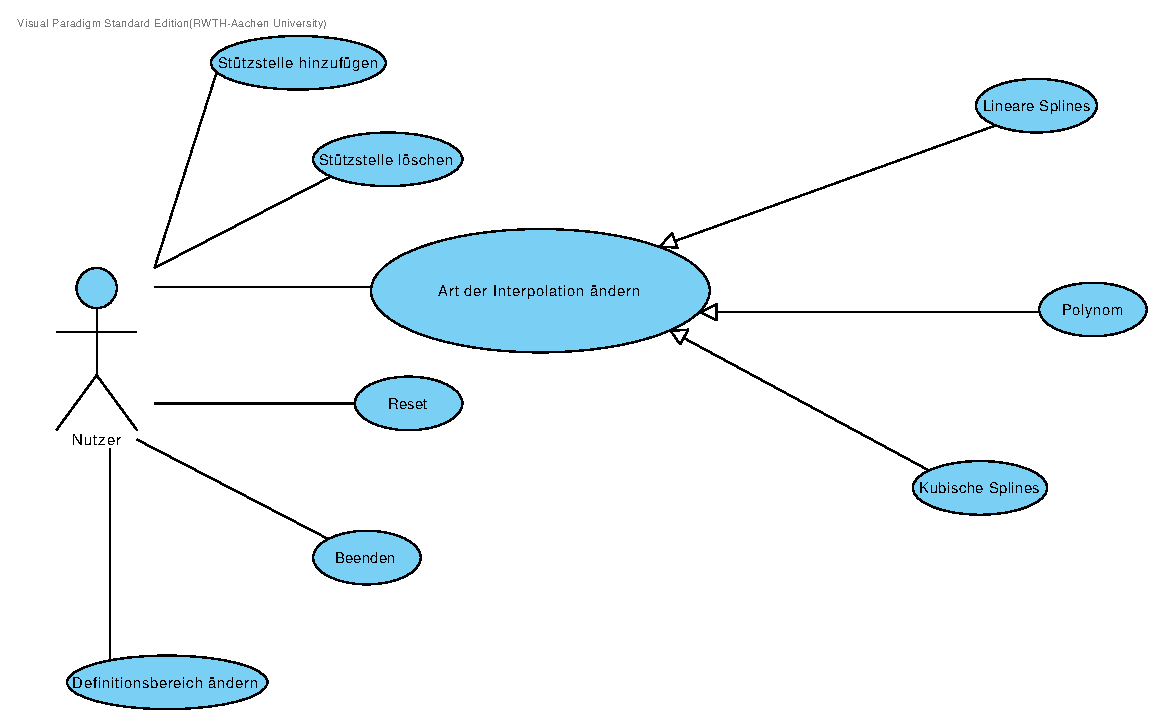
\includegraphics[width=\textwidth]{Aktivitaetsdiagramm/Top_Level_Use_Cases}
\caption{Anwendungsfalldiagramm}
\label{fig:Anwendungsfalldiagramm}
\end{figure}

\textbf{Aktivit\"atsdiagramme:}

\textbf{Art der Interpolation \"andern}
  \begin{itemize}
  \item \textit{Ziel:} Der Nutzer will die Interpolationsart \"andern.
  \item \textit{Einordnung:} Hauptfunktion
  \item \textit{Vorbedingung:} Die Applikation ist ge\"offnet und zeigt die Zeichenfl\"ache sowie die Benutzeroberfl\"ache an.
  \item \textit{Nachbedingung:} Die Applikation zeigt die neu berechnete Kurve auf der Zeichenfl\"ache an.
  \item \textit{Nachbedingung im Fehlerfall:} 
  \item \textit{Hauptakteure:} Nutzer
  \item \textit{Nebenakteure:} 
  \item \textit{Ausl\"oser:} Der Nutzer will die Interpolationsart \"andern.
  \item \textit{Standardablauf:}
    \begin{enumerate}[label=(\arabic*)]
    \item Der Nutzer klickt mit der linken Maustaste auf die Auswahlbox mit der \"Uberschrift "'Interpolationsart", welche sich auf der Benutzeroberfl\"ache befindet.
    \item Die Applikation zeigt alle m\"oglichen Interpolationsmethoden in der Auswahlbox an.
    \item Der Nutzer w\"ahlt mit der linken Maustaste eine Interpolationsart aus.
    \item Die Applikation f\"uhrt die Interpolation mit der ausgew\"ahlten Interpolationsmethode aus.
    \item Die Applikation zeigt die neu berechnete Interpolation auf der Zeichenfl\"ache an.
    \end{enumerate}
  \end{itemize}

\begin{figure}[H]
\centering
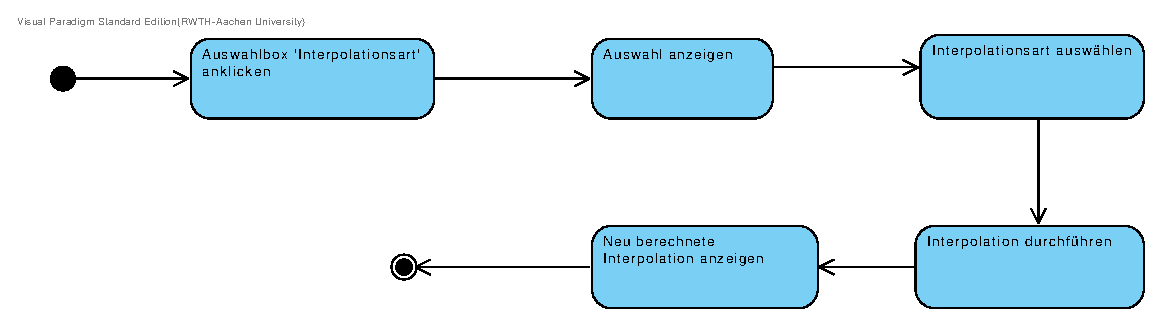
\includegraphics[width=\textwidth]{Aktivitaetsdiagramm/interpolationAuswaehlen.eps}
\caption{Interpolationsart aendern}
\label{fig:Interpolationsart aendern}
\end{figure}

\hfill \\
\hfill \\
\textbf{Reset}
  \begin{itemize}
  \item \textit{Ziel:} Es sollen alle St\"utzstellen und die Kurve von der Zeichenfl\"ache gel\"oscht, sowie der Definitionsbereich und die Interpolationsart auf den Defaultmodus (Lineare Spline Interpolation ([0,100]x[0,50]) zur\"uckgesetzt werden.
  \item \textit{Einordnung:} Hauptfunktion
  \item \textit{Vorbedingung:} Die Applikation ist ge\"offnet und zeigt die Zeichenfl\"ache sowie die Benutzeroberfl\"ache an.
  \item \textit{Nachbedingung:} Die Applikation hat alle St\"utzstellen auf der Zeichenfl\"ache gel\"oscht und der Definitionsbereich sowie die Interpolationsart sind im Defaultmodus.
  \item \textit{Nachbedingung im Fehlerfall:} 
  \item \textit{Hauptakteure:} Nutzer
  \item \textit{Nebenakteure:}
  \item \textit{Ausl\"oser:} Der Nutzer m\"ochte die Applikation auf den Defaultmodus zur\"ucksetzen.
  \item \textit{Standardablauf:}
    \begin{enumerate}[label=(\arabic*)]
    \item Der Nutzer klickt mit der linken Maustaste auf den Button 'Reset', welcher sich auf der Benutzeroberfl\"ache befindet.
    \item Die Applikation stellt den Defaultmodus wieder her und l\"oscht die St\"utzstellen.
   % \item Die Applikation entfernt alle St\"utzstellen.							%Sollen die Aktivit\"aten des Systemes angezeigt werden?
    %\item Die Applikation ruft den UC Case Interpolieren auf
   %\item Die Applikation setzt den Definitionsbereich auf [0,50]x[0,100].
  %  \item Die Applikation setzt die Interpolationsart auf  'Lineare Splines'.
    
    \end{enumerate}
 \end{itemize}  
\begin{figure}[H]
\centering
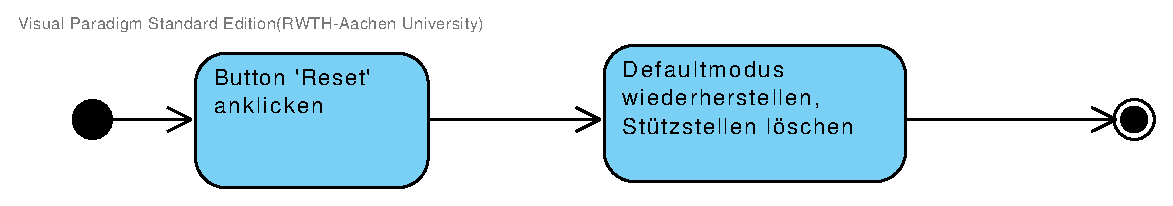
\includegraphics[width=\textwidth]{Aktivitaetsdiagramm/Reset.eps}
\caption{Reset}
\label{fig:Reset}
\end{figure}

\hfill \\
\hfill \\
\textbf{Definitionsbereich \"andern}
  \begin{itemize}
  \item \textit{Ziel:} Der Definitionsbereich soll ge\"andert werden
  \item \textit{Einordnung:}  Hauptfunktion
  \item \textit{Vorbedingung:} Die Applikation ist ge\"offnet und zeigt die Zeichenfl\"ache sowie die Benutzeroberfl\"ache an.
  \item \textit{Nachbedingung:} Die Applikation zeigt die aktualisierte Zeichenfl\"ache sowie Benutzeroberfl\"ache mit den neuen Grenzen an.
  \item \textit{Nachbedingung im Fehlerfall:} Die Applikation zeigt eine Fehlermeldung an und ver\"andert die Zeichenfl\"ache nicht.
  \item \textit{Hauptakteure:} Nutzer
  \item \textit{Nebenakteure:}
  \item \textit{Ausl\"oser:} Der Nutzer will den Definitionsbereich \"andern
  \item \textit{Standardablauf:}
    \begin{enumerate}[label=(\arabic*)]
    \item Der Nutzer klickt mit der linken Maustaste auf eins der Textfelder auf der Benutzeroberfl\"ache unter der \"Uberschrift "'Definitionsbereich".
    \item Der Nutzer \"andert den Wert im Textfeld.
    \item Der Nutzer bet\"atigt mit der linken Maustaste den Button 'Definitionsbereich setzen'.
    \item Die Applikation pr\"uft, ob Zahlen eingegeben wurden.
    \item Die Applikation pr\"uft, ob $ x_{min} > x_{max}$ ist. 
    \item Die Applikation pr\"uft, ob $ y_{min} > y_{max}$ ist.
    \item Die Applikation \"andert den Definitionsbereich auf die gew\"unschten Werte.
    \end{enumerate}
      \item \textit{Verzweigungen:}
     \begin{enumerate}[label=(2a\arabic*)]            	\setcounter{enumii}{3}
      \item Der Nutzer will noch einen anderen Wert des Definitionsbereiches \"andern.
   	\item Der Nutzer geht zu Schritt '1' zur\"uck.
                \end{enumerate}      
    \begin{enumerate}[label=(4a\arabic*)]
      \item Der Nutzer hat eine ung\"ultige Eingabe get\"atigt.
      \item Die Applikation gibt eine Fehlermeldung aus.
      \end{enumerate}
                      \begin{enumerate}[label=(5a\arabic*)]
    \setcounter{enumii}{4}
    \item Die Applikation erkennt, dass  '$ x_{min} > x_{max}$'  ist.
      \item Die Applikation gibt eine Fehlermeldung aus.
      \end{enumerate}
           \begin{enumerate}[label=(6a\arabic*)]
     \setcounter{enumii}{5}
    \item Die Applikation erkennt, dass  '$ y_{min} > y_{max}$'  ist.
    \item Die Applikation gibt eine Fehlermeldung aus.
      \end{enumerate}
  \end{itemize}

\begin{figure}[H]
\centering
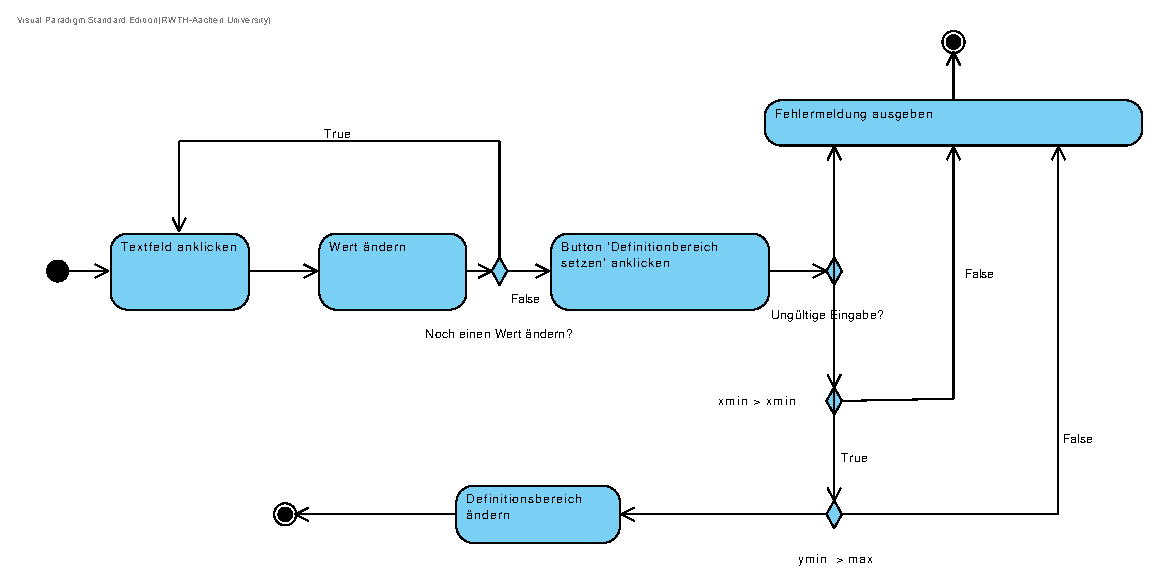
\includegraphics[width=\textwidth]{Aktivitaetsdiagramm/definitionbereichAendern.eps}
\caption{Definitionsbereich aendern}
\label{fig:Definitionsbereich aendern}
\end{figure}

\hfill \\
\hfill \\
\textbf{Beenden}
  \begin{itemize}
  \item \textit{Ziel:} Die Applikation soll beendet werden
  \item \textit{Einordnung:} Hauptfunktion
  \item \textit{Vorbedingung:} Die Applikation ist ge\"offnet und zeigt die Zeichenfl\"ache sowie die Benutzeroberfl\"ache an.
  \item \textit{Nachbedingung:} Die Applikation wurde erfolgreich beendet.
  \item \textit{Nachbedingung im Fehlerfall:} 
  \item \textit{Hauptakteure:} Nutzer
  \item \textit{Nebenakteure:}
  \item \textit{Ausl\"oser:} Der Nutzer m\"ochte die Applikation beenden.
    \item \textit{Standardablauf:}
    \begin{enumerate}[label=(\arabic*)]
    \item Der Nutzer bet\"atigt auf der Benutzeroberfl\"ache mit der linken Maustaste den Button 'Beenden'.
    \item Die Applikation schlie\ss t.
    \end{enumerate}
 \end{itemize}  
\begin{figure}[H]
\centering
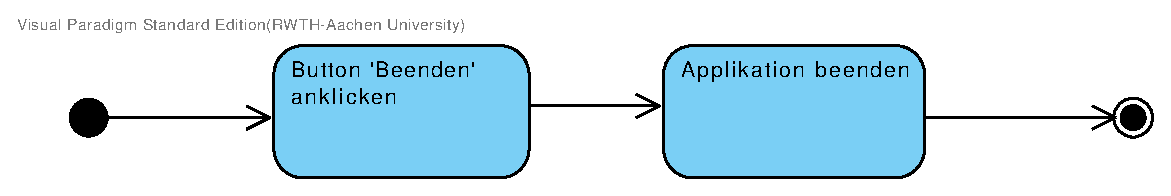
\includegraphics[width=\textwidth]{Aktivitaetsdiagramm/beenden.eps}
\caption{Beenden}
\label{fig:Beenden}
\end{figure}

\hfill \\
\hfill \\
\textbf{St\"utzstelle l\"oschen}
  \begin{itemize}
  \item \textit{Ziel:} Es soll eine vom Nutzer angeklickte St\"utzstelle von der Zeichenfl\"ache gel\"oscht werden.
  \item \textit{Einordnung:} Hauptfunktion
  \item \textit{Vorbedingung:} Die Applikation ist ge\"offnet und zeigt die Zeichenfl\"ache sowie die Benutzeroberfl\"ache an.
  \item \textit{Nachbedingung:} Die Applikation zeigt die neu berechnete Interpolation ohne die gel\"oschte St\"utzstelle auf der Zeichenfl\"ache an.
  \item \textit{Nachbedingung im Fehlerfall:}  Die Applikation zeigt die urspr\"ungliche Interpolation an.
  \item \textit{Hauptakteure:} Nutzer
  \item \textit{Nebenakteure:} 
  \item \textit{Ausl\"oser:} Der Nutzer m\"ochte eine St\"utzstelle von der Zeichenfl\"ache l\"oschen
  \item \textit{Standardablauf:}
    \begin{enumerate}[label=(\arabic*)]
    \item Der Nutzer klickt mit der rechten Maustaste auf eine beliebige Stelle der Zeichenfl\"ache.
    \item Die Applikation l\"oscht die im L\"oschradius befindliche St\"utzstelle mit dem kleinsten x-Wert.
    \item Die Applikation f\"uhrt die Interpolation mit den verbleibenden St\"utzstellen aus.
    \item Die Applikation zeigt die neu berechnete Interpolation auf der Zeichenfl\"ache an.
   
    \end{enumerate}
  \item \textit{Verzweigungen:}
    \begin{enumerate}[label=(\arabic*a)]
    \setcounter{enumii}{1}
      \item Die Applikation kann keine St\"utzstelle im L\"oschradius identifizieren.
      \item Der Use Case wird beendet.
      \end{enumerate}

 \end{itemize}

\begin{figure}[H]
\centering
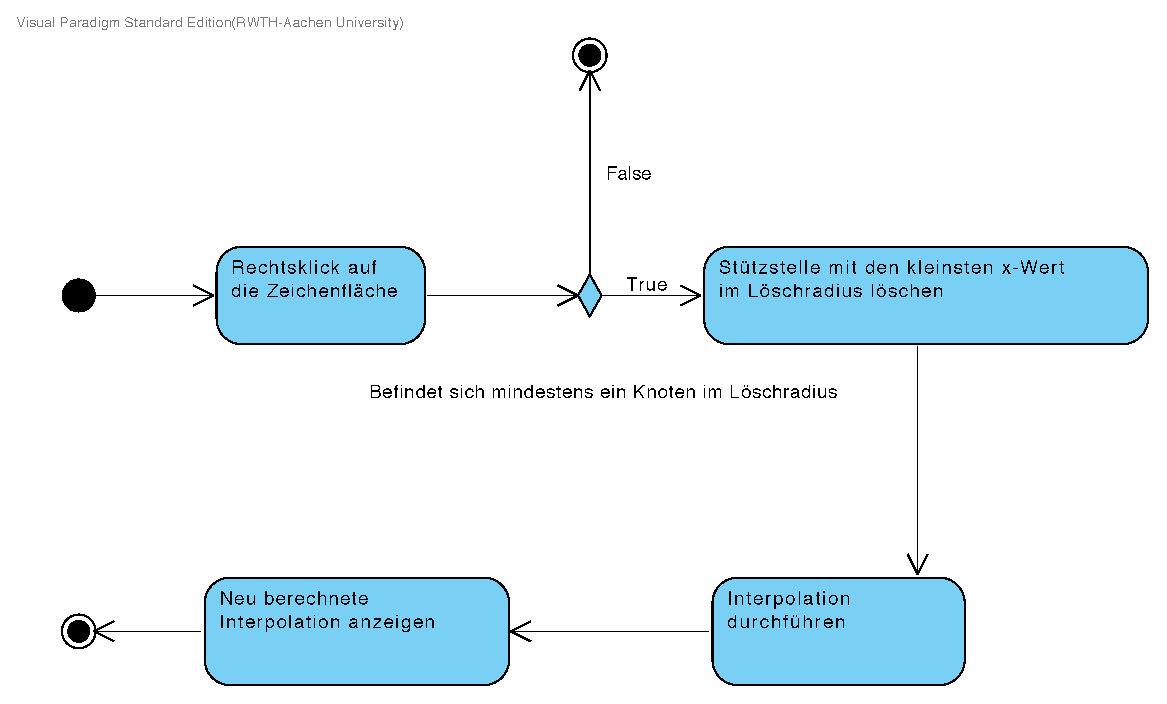
\includegraphics[width=\textwidth]{Aktivitaetsdiagramm/stuetzstelleLoeschen.eps}
\caption{Stuetzstelle loeschen}
\label{fig:Stutzstelle loeschen}
\end{figure}

\hfill \\
\hfill \\
\textbf{St\"utzstelle hinzuf\"ugen}
  \begin{itemize}
  	\item \textit{Ziel:} Die Interpolation soll um eine St\"utzstelle erweitert werden.
  	\item \textit{Einordnung:} Hauptfunktion
  	\item \textit{Vorbedingung:} Die Applikation ist ge\"offnet und zeigt die Zeichenfl\"ache sowie die Benutzeroberfl\"ache an.
  	\item \textit{Nachbedingung:} Die Applikation zeigt die neu berechnete Interpolation mit der hinzugef\"ugten St\"utzstelle auf der Zeichenfl\"ache an.
  \item \textit{Nachbedingung im Fehlerfall:} 
  \item \textit{Hauptakteure:} Nutzer
  \item \textit{Nebenakteure:} 
  \item \textit{Ausl\"oser:} Der Nutzer m\"ochte eine St\"utzstelle auf der Zeichenfl\"ache hinzuf\"ugen.
  \item \textit{Standardablauf:}
    \begin{enumerate}[label=(\arabic*)]
    \item Der Nutzer klickt mit der linken Maustaste auf eine beliebige Stelle der Zeichenfl\"ache.
    \item Die Applikation erzeugt eine St\"utzstelle auf dem angeklickten Punkt.
    \item Die Applikation f\"uhrt die Interpolation mit den neuen St\"utzstellen aus.
    \item Die Applikation zeigt die neu berechnete Interpolation auf der Zeichenfl\"ache an.
    \end{enumerate}
  \end{itemize}

\begin{figure}[H]
\centering
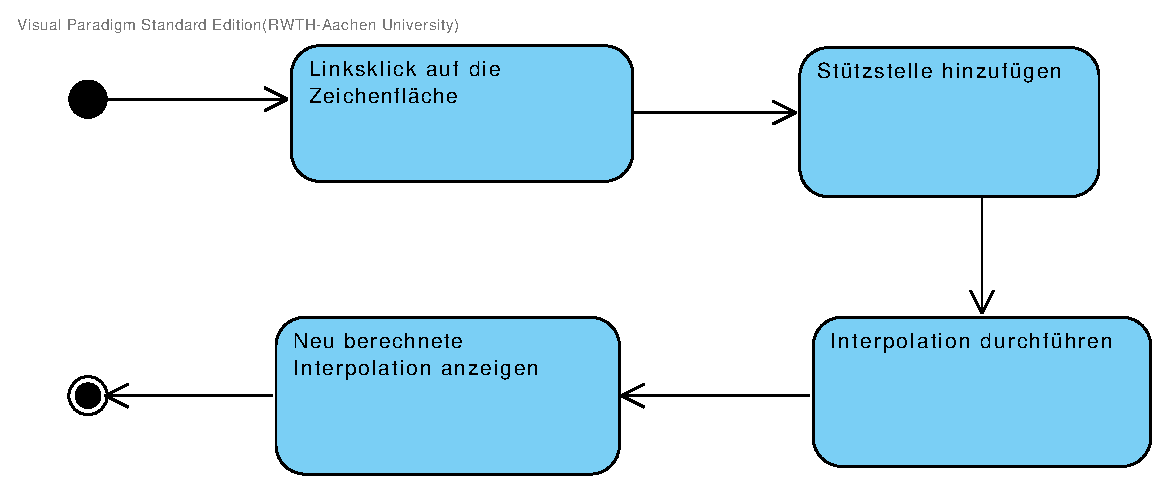
\includegraphics[width=\textwidth]{Aktivitaetsdiagramm/stutzstelleHInzufuegen.eps}
\caption{Stuetzstelle hinzufuegen}
\label{fig:Stuetzstelle hinzufuegen}
\end{figure}



\section{Systemanforderungen}

\subsection{Funktionale Anforderung}
\begin{itemize}
\item Anzeigen einer Zeichenfl\"ache
\item Anzeigen einer Benutzeroberfl\"ache, welche folgende Funktionen bereitstellt:
	\begin{enumerate}
	\item Auswahl der Interpolationmethode
	\item \"Anderung des Definitionsbereichs
	\item Zur\"ucksetzten der Zeichenfl\"ache und Einstellungen auf default
	\item Beenden Button
	\end{enumerate}
\item Anzeigen von Fehlermeldungen
\item Eingabe von Gleitkommazahlen 
\item Anzeigen einer Interpolationskurve
\item Darstellung von Punkten auf der Zeichenfl\"ache
\item Speichern der Punkte (Gleitkommazahlen, ganze Zahlen)
\item L\"oschen und Hinzuf\"ugen von Punkten
\item Test auf G\"ultigkeit des Definitionsbereichs
\item Anzeigen von Gleitkommazahlen auf 2 Nachkommastellen 
\item Nach dem Starten des Programms werden Defintionsbereich und Interpolationsart standardm\"a\ss ig fesgelegt
\end{itemize}
\subsection{Nicht Funktionale Anforderung}
\begin{itemize}
\item Hinzuf\"ugen und L\"oschen der Punkte durch Mausklick m\"oglich
\item Eingabe der Zahlen durch Tastatur
\item Skalierung des Hauptfensters bei unterschiedlichen Aufl\"osungen.
\end{itemize}


\section{Begriffsanalyse}
\textbf{Klassenkandidaten:}
\begin{itemize}
  \item \textbf{Zeichenfl\"ache}
  \item \textbf{Benutzeroberfl\"ache}
  \item Definitionsbereich
  \item \textbf{Interpolationsart}
  \item Button
  \item Textfeld
  \item Auswahlbox
  \item \textbf{MainWindow}
  \item St\"utzstelle
  \item L\"oschradius
\end{itemize}
\textbf{Begriffsmodell:}

\begin{figure}
\centering
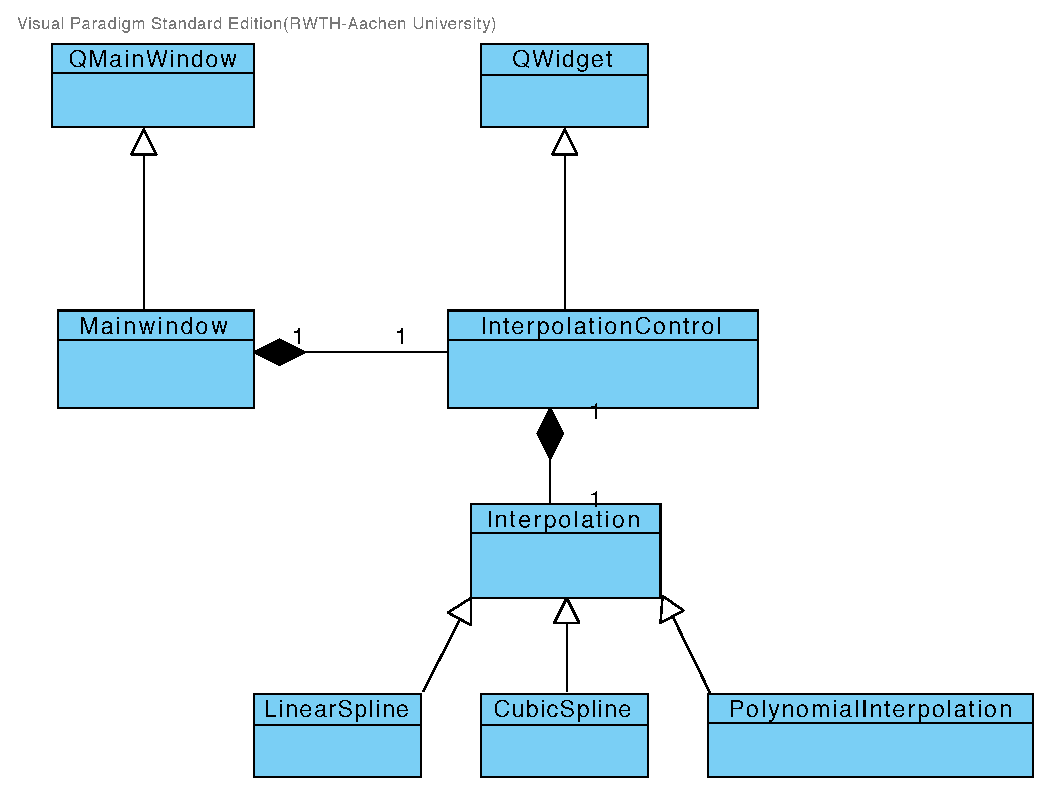
\includegraphics[width=\textwidth]{figures/Begriffsmodel.eps}
\caption{Begriffsmodell}
\end{figure}

\chapter{Entwurf}
\label{ch:3}

\section{Detailentwurf: Klassen}
\label{sec:3.1}

\subsection{Statik}
\begin{figure}[!htb]
\centering
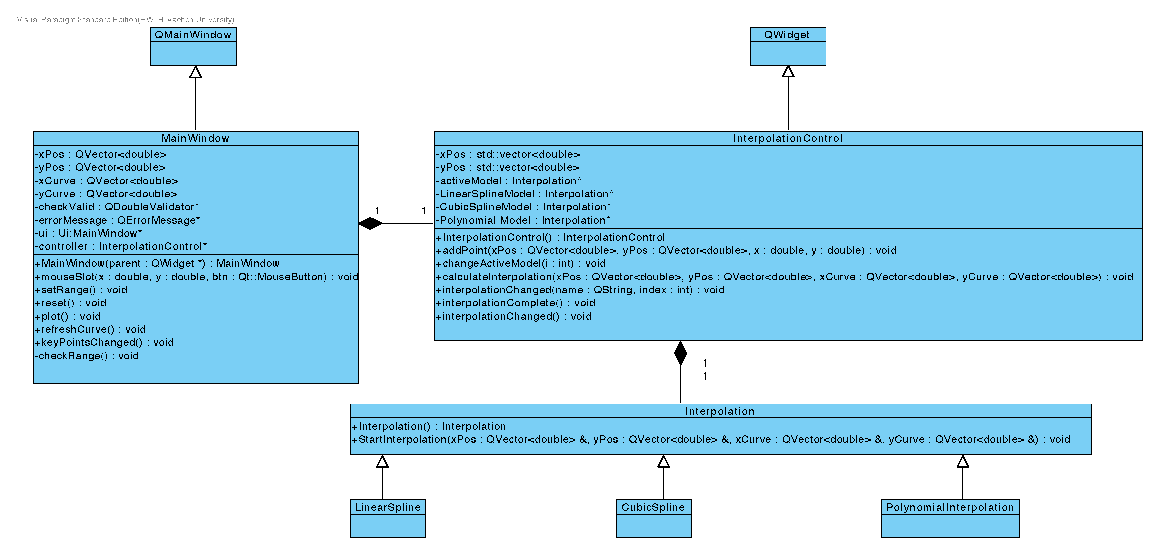
\includegraphics[width=\textwidth]{figures/klassendiagramm.eps}
\caption{Klassendiagramm}
\label{fig:Klassendiagramm}
\end{figure}

\subsection{Dynamik}

\begin{figure}
\centering
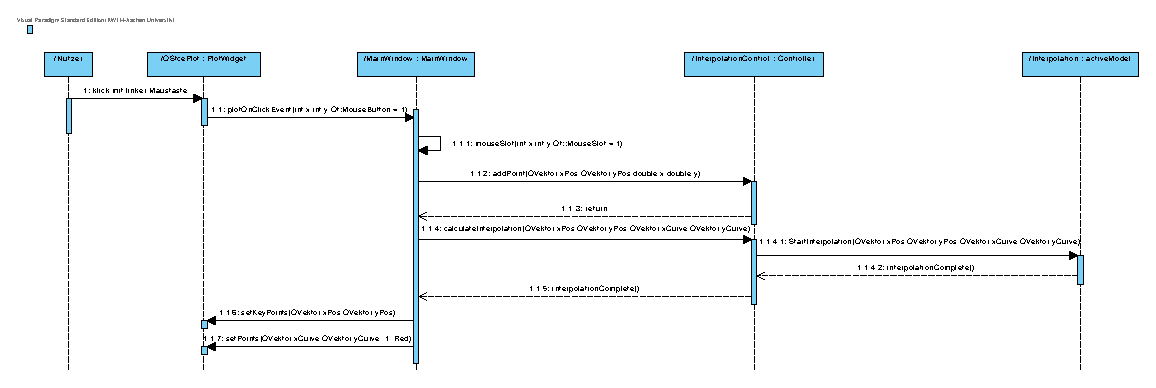
\includegraphics[width=\textwidth]{figures/sequenzdiagramme/mausklick_links_auf_zeichenflaeche.eps}
\caption{Sequenzdiagramm: Stuetzstelle hinzufuegen}
\end{figure}

\begin{figure}
\centering
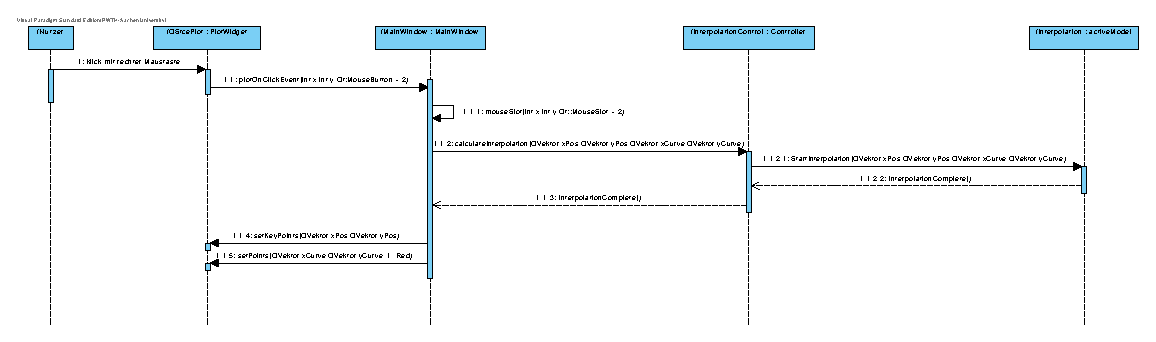
\includegraphics[width=\textwidth]{figures/sequenzdiagramme/mausklick_rechts_auf_zeichenflaeche.eps}
\caption{Sequenzdiagramm: Stuetzstelle loeschen}
\end{figure}

\begin{figure}
\centering
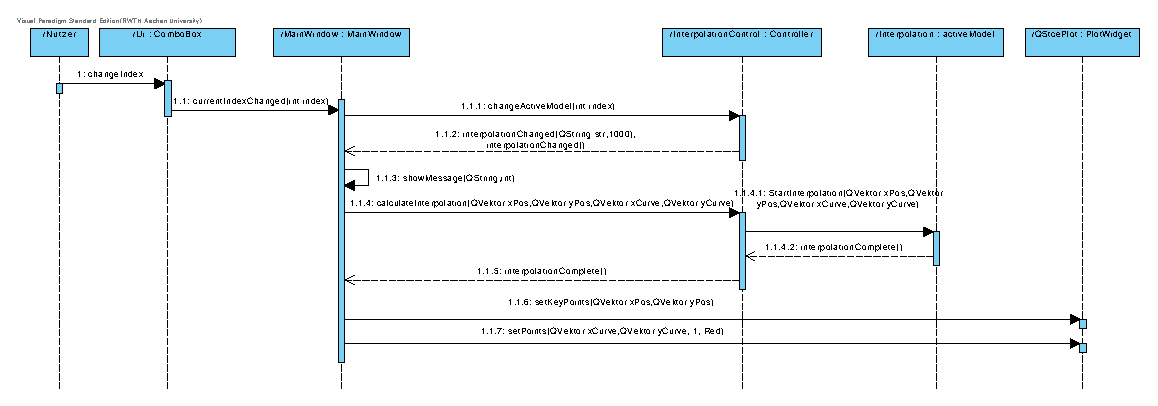
\includegraphics[width=\textwidth]{figures/sequenzdiagramme/interpolation_aendern.eps}
\caption{Sequenzdiagramm: Interpolationsart aendern}
\end{figure}

\begin{figure}
\centering
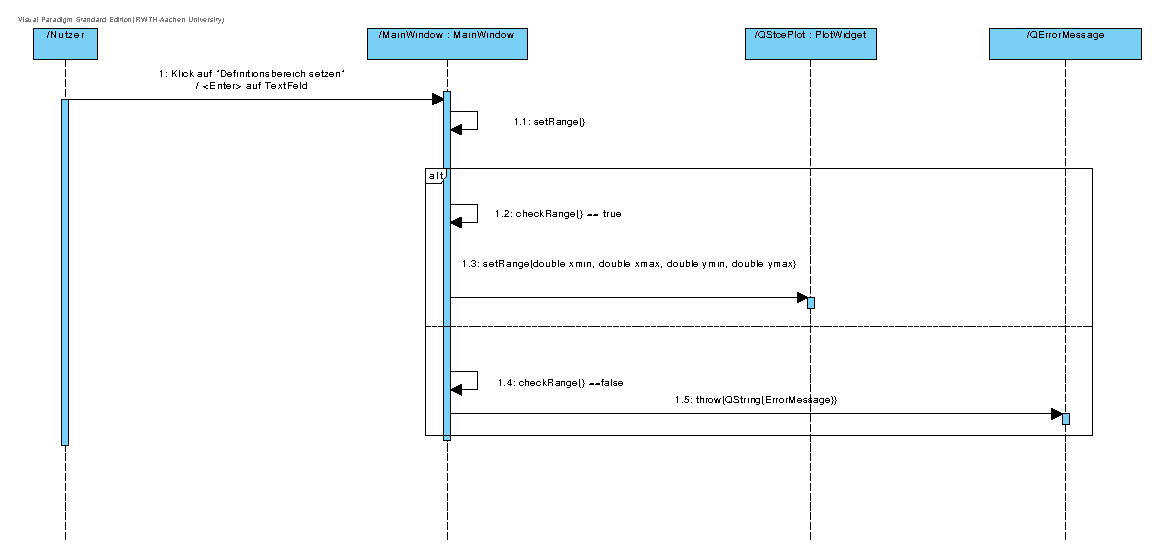
\includegraphics[width=\textwidth]{figures/sequenzdiagramme/definitionsbereich_aendern.eps}
\caption{Sequenzdiagramm: Definitionsbereich aendern}
\end{figure}

\begin{figure}
\centering
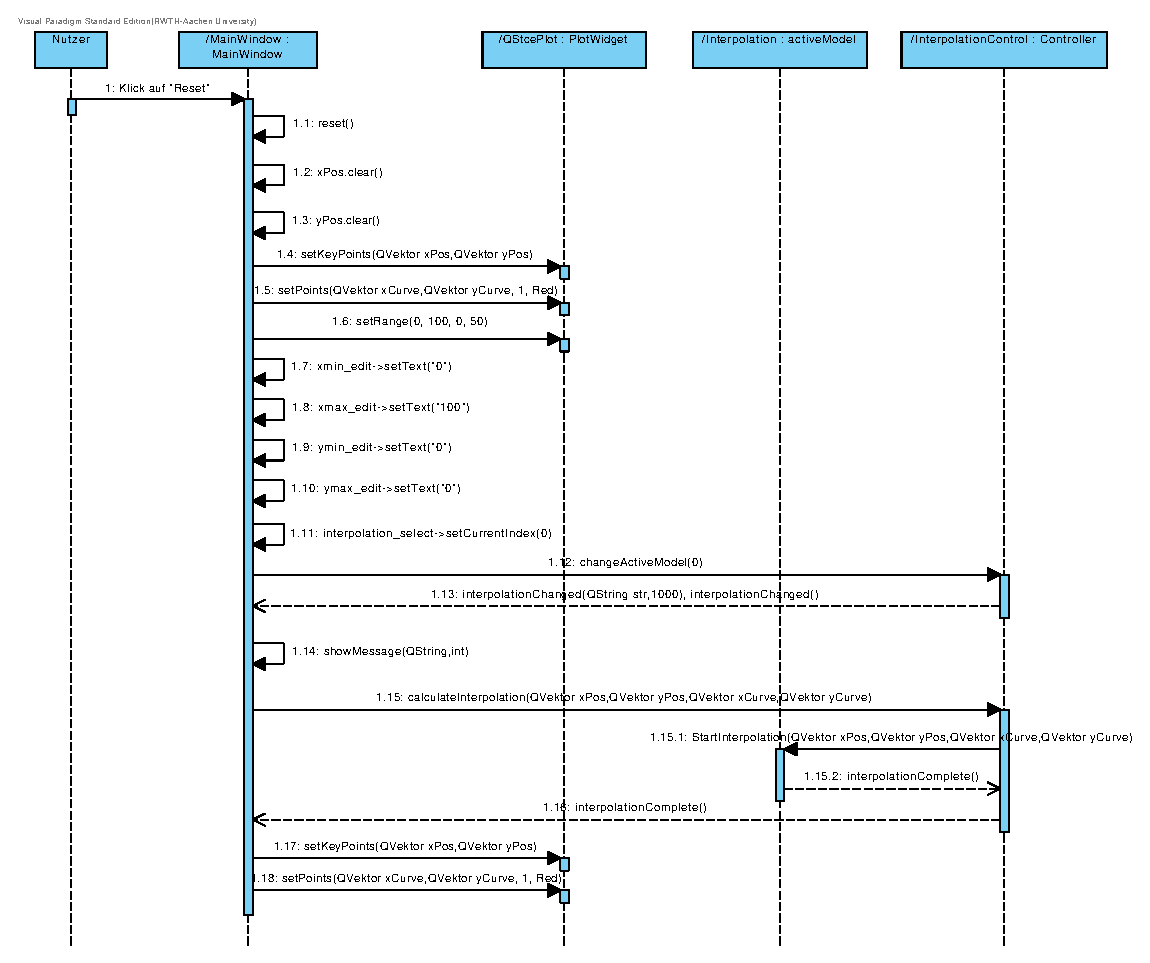
\includegraphics[width=\textwidth]{figures/sequenzdiagramme/Reset.eps}
\caption{Sequenzdiagramm: Reset}
\end{figure}

\begin{figure}
\centering
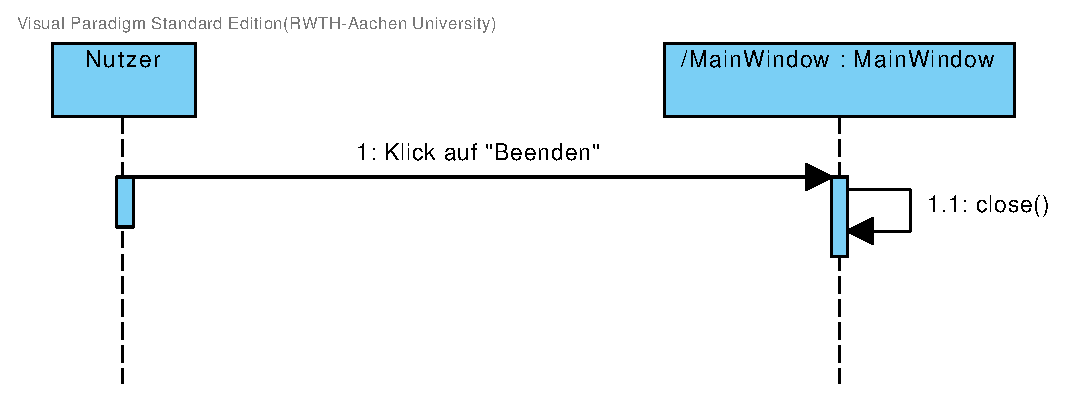
\includegraphics[width=\textwidth]{figures/sequenzdiagramme/Beenden.eps}
\caption{Sequenzdiagramm: Beenden}
\end{figure}
\chapter{Benutzerdokumentation}
\label{ch:4}

\section{Installation}
\subsection{Voraussetzungen}
F\"ur die Installation der Software ist ein Linux basiertes Betriebssystem, sowie die Vorinstallation von QT (Version 5) notwendig.

\subsection{Unkompilierte Version}
F\"ur die Installation der unkompilierten Version sind folgende Schritte zu befolgen:
\begin{enumerate}
  \item Erstellen eines gew\"unschten Installationsverzeichnisses, z.B. \verb+./Interpolation+
  \item Speichern von \verb+Interpolation.zip+ in dem gew\"ahlten Verzeichnis.
  \item Entpacken des Archivs mittels \verb+unzip Interpolation.zip+ oder einer entsprechenden Software.
  \item Ausf\"uhren von \verb+qmake-qt5+ in dem gew\"ahlten Verzeichnis.
  \item Anschlie\ss end ausf\"uhren von \verb+make+ in dem gleichen Verzeichnis.
  \item 'make clean' stellt den Ausgangszustand des Programms wieder her, erh\"alt aber die ausf\"uhrbare Datei.
  \item Ausf\"uhren des Programms durch das Starten der ausf\"uhrbaren Datei 'Interpolation'.
\end{enumerate}

\section{Beispielsitzung}
Das Programm startet mit der Anzeige des Hauptfensters.\\

\begin{figure}[H]
\centering
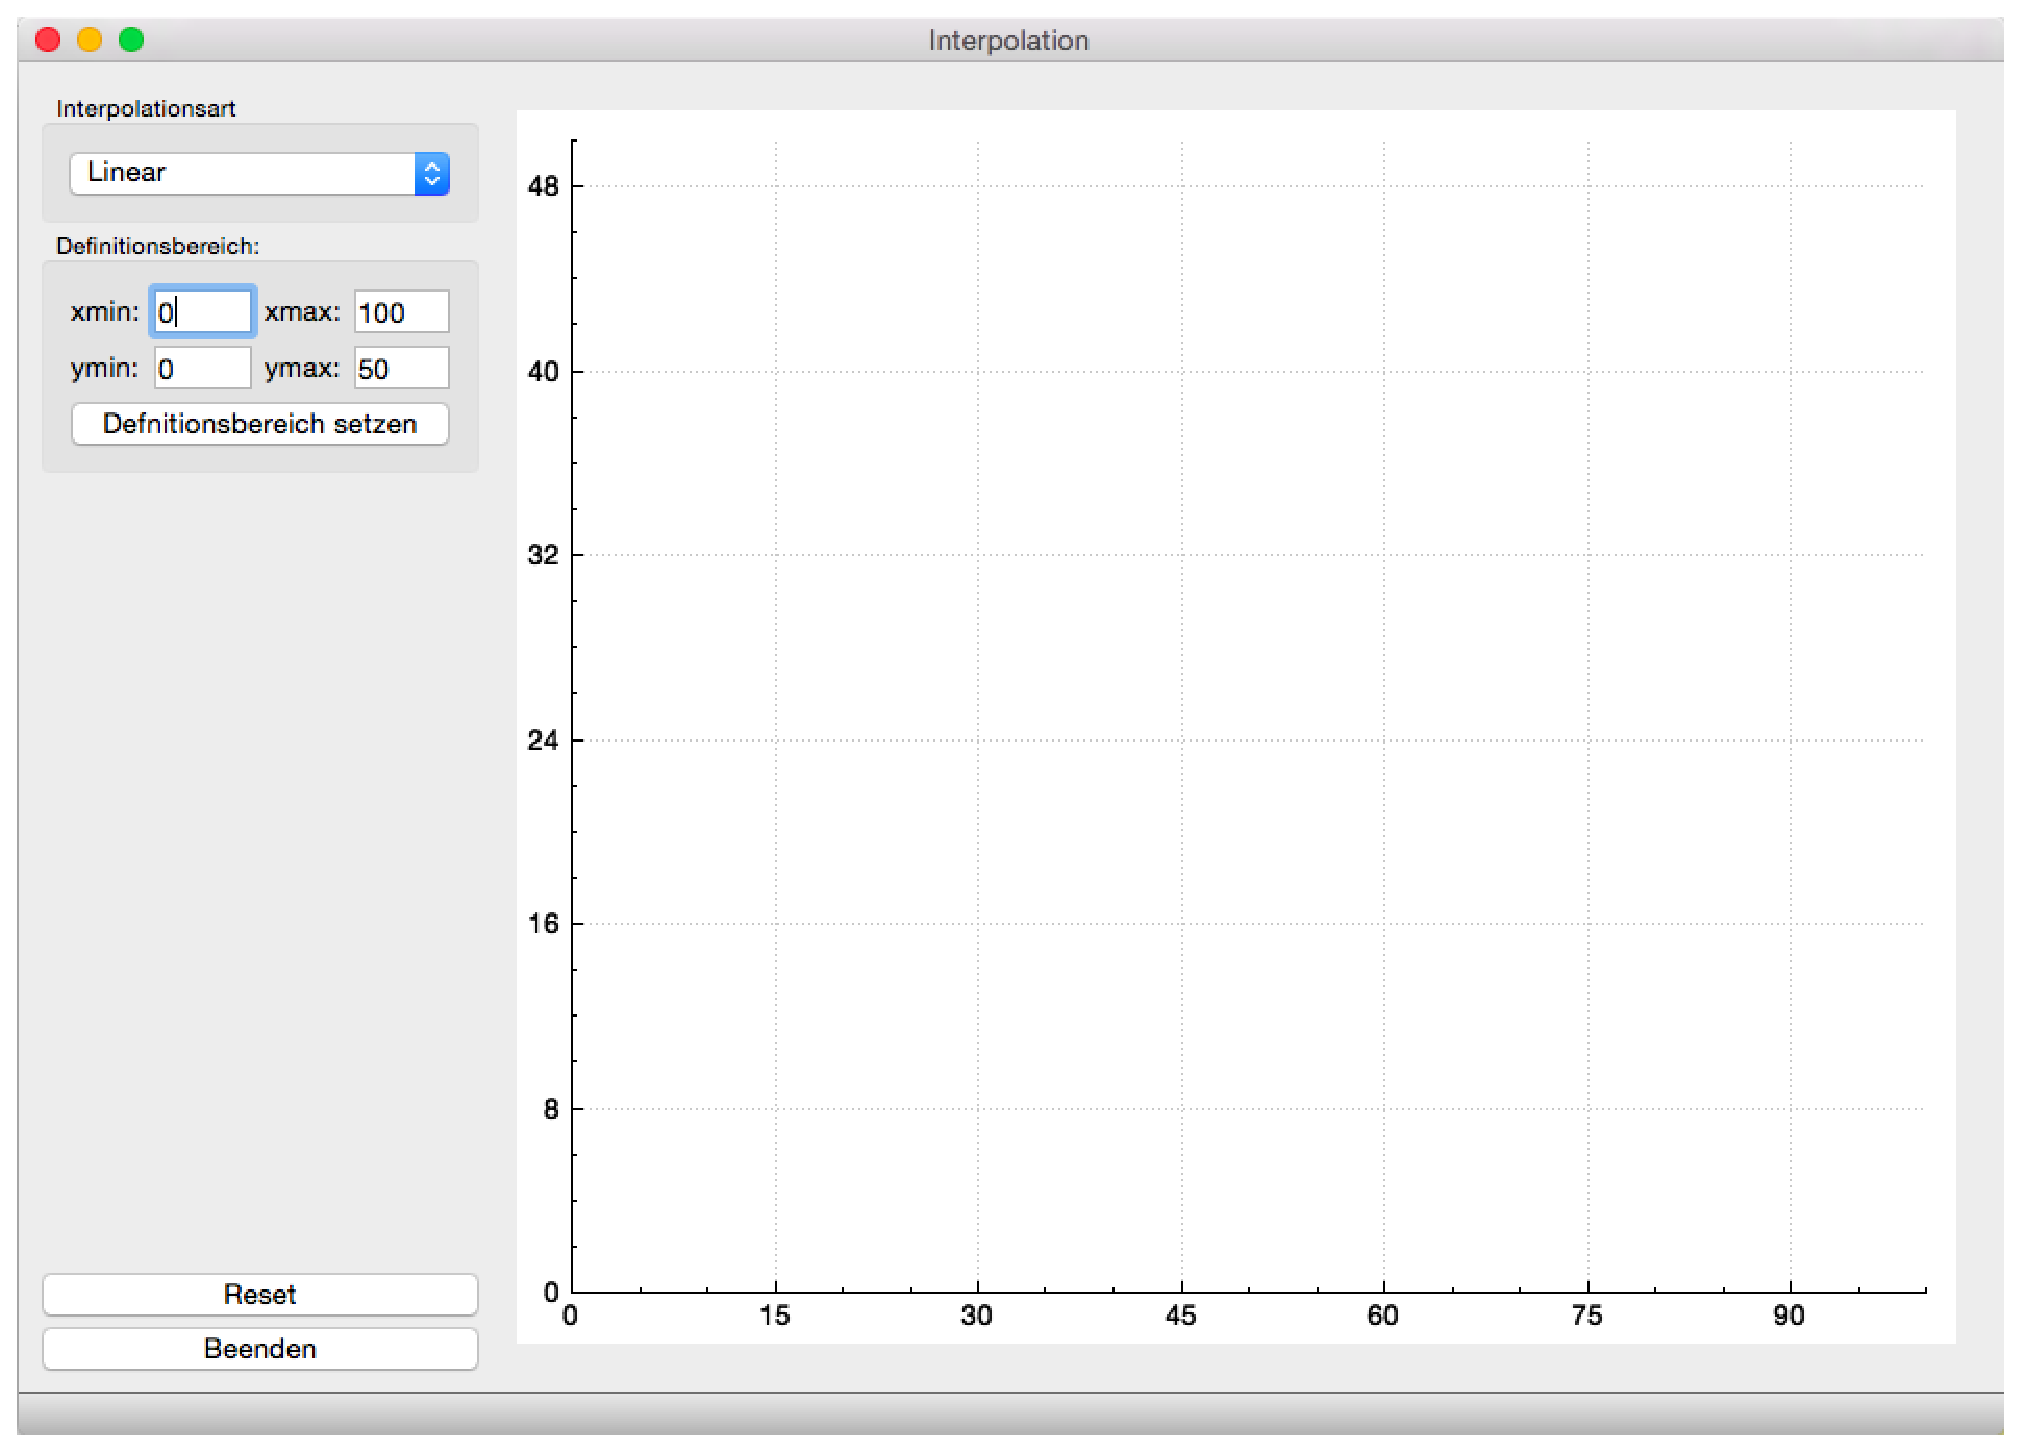
\includegraphics[width=\textwidth]{figures/start_screen.eps}
\caption{Startbildschirm}
\end{figure}

\noindent Der Nutzer klickt auf die Zeichenfl\"ache mehrmals um Punkte hinzuzuf\"ugen. Diese werden auf der Zeichenfl\"ache direkt angezeigt und durch gerade Linien (lineare Splines) verbunden.\\

\begin{figure}[H]
\centering
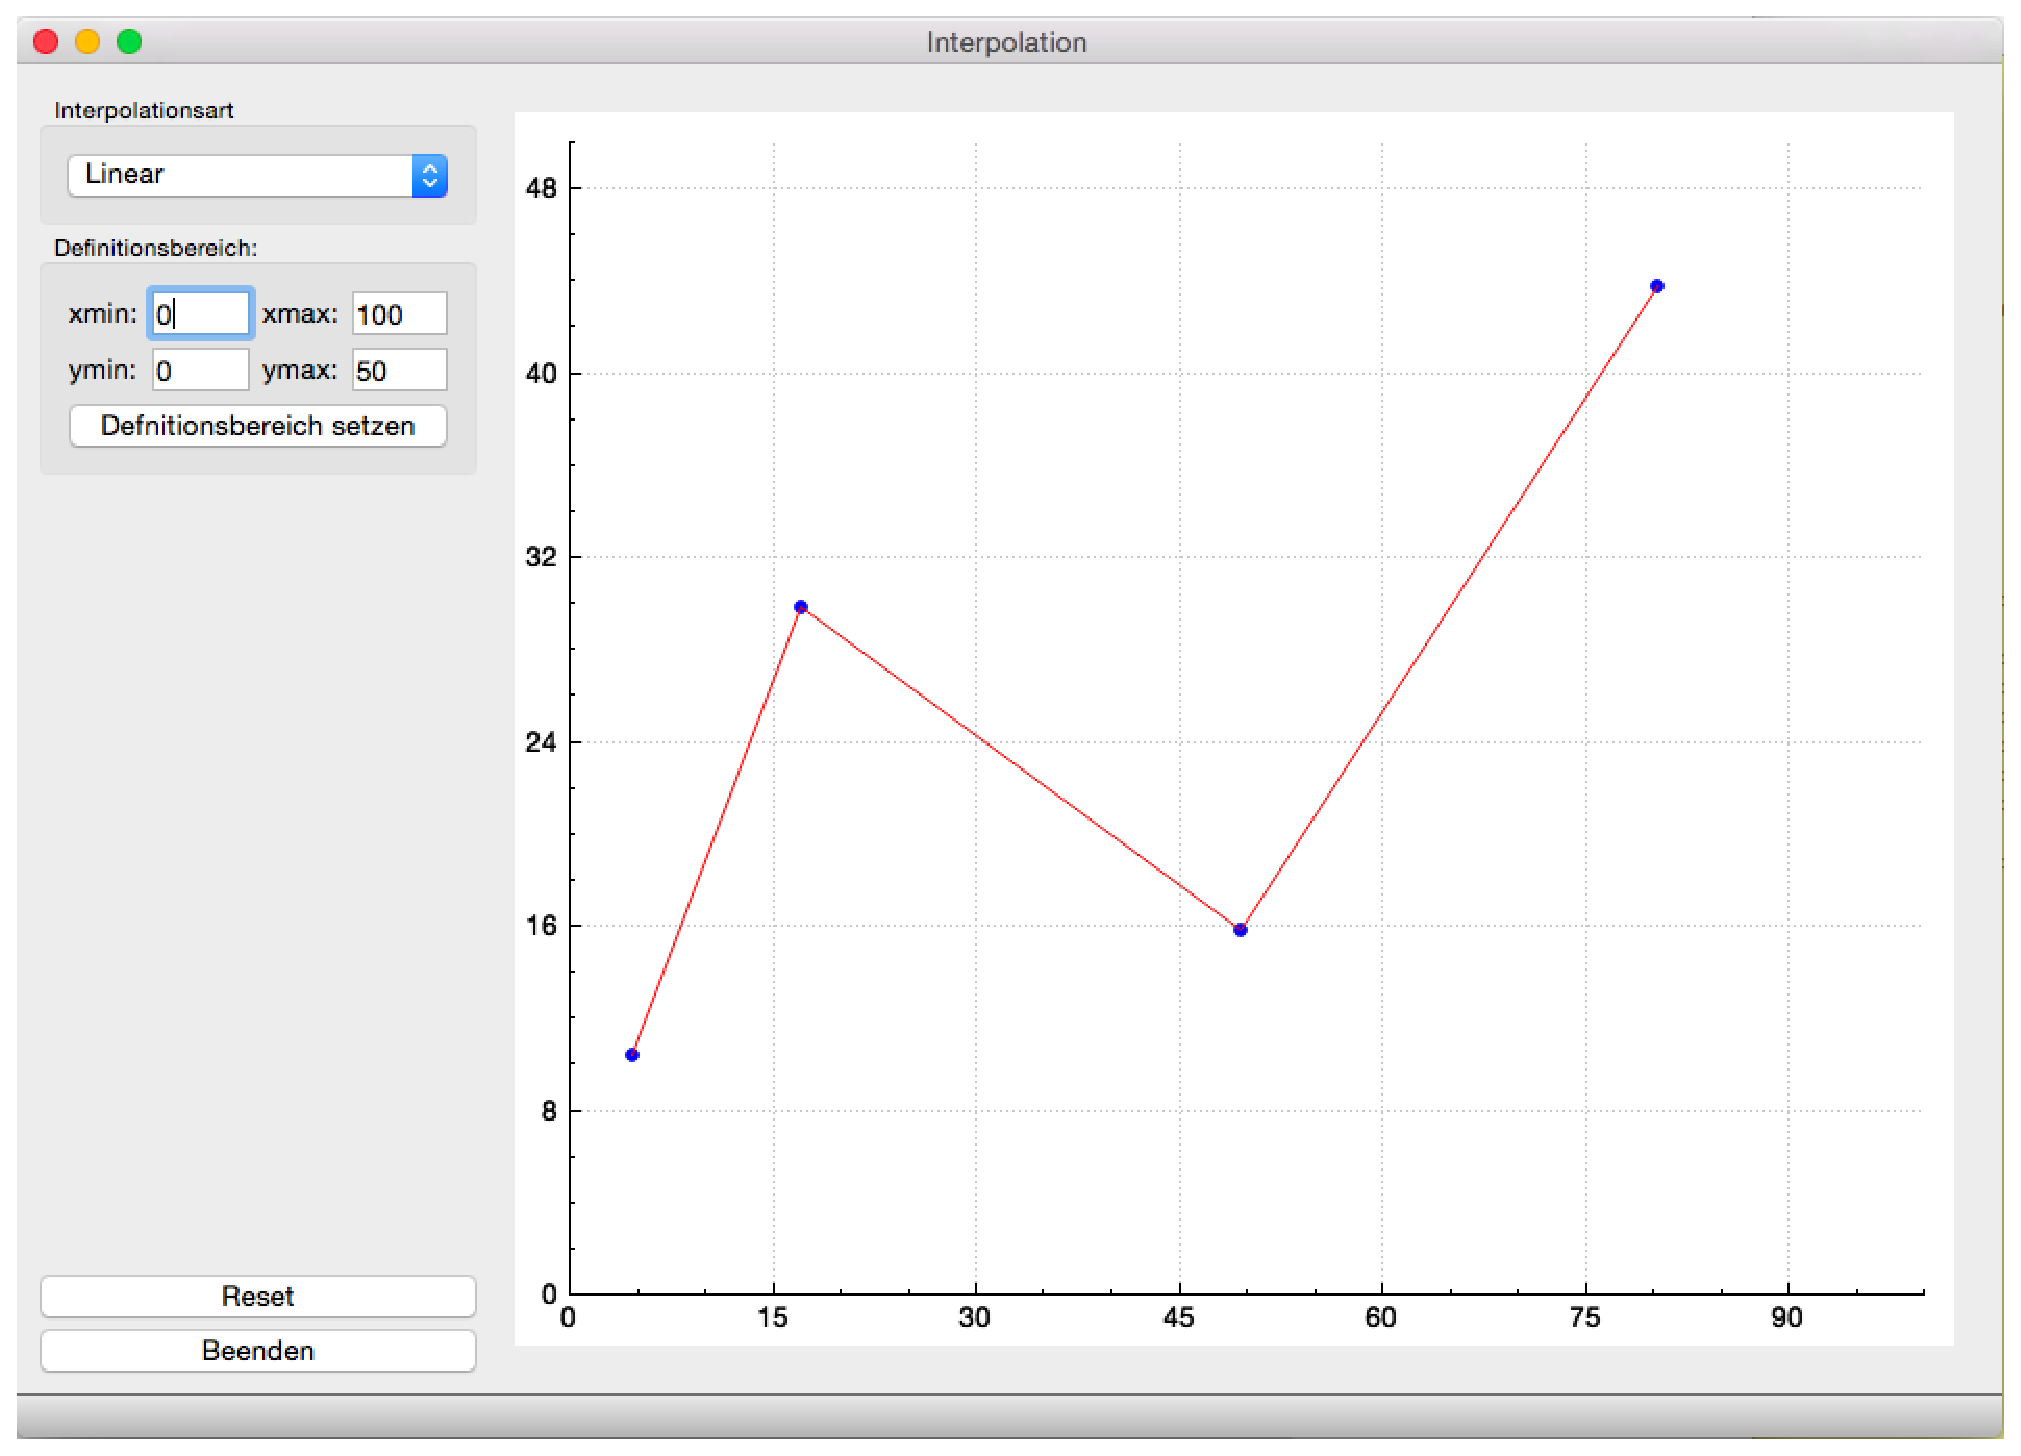
\includegraphics[width=\textwidth]{figures/linear_interpol_screen.eps}
\caption{Lineare Interpolation zwischen Punkten}
\end{figure}

\noindent Der Nutzer w\"ahlt die Interpolationsart 'Polynominterpolation' aus. Die Punkte werden nun durch eine Polynomkurve miteinander verbunden.\\

\begin{figure}[H]
\centering
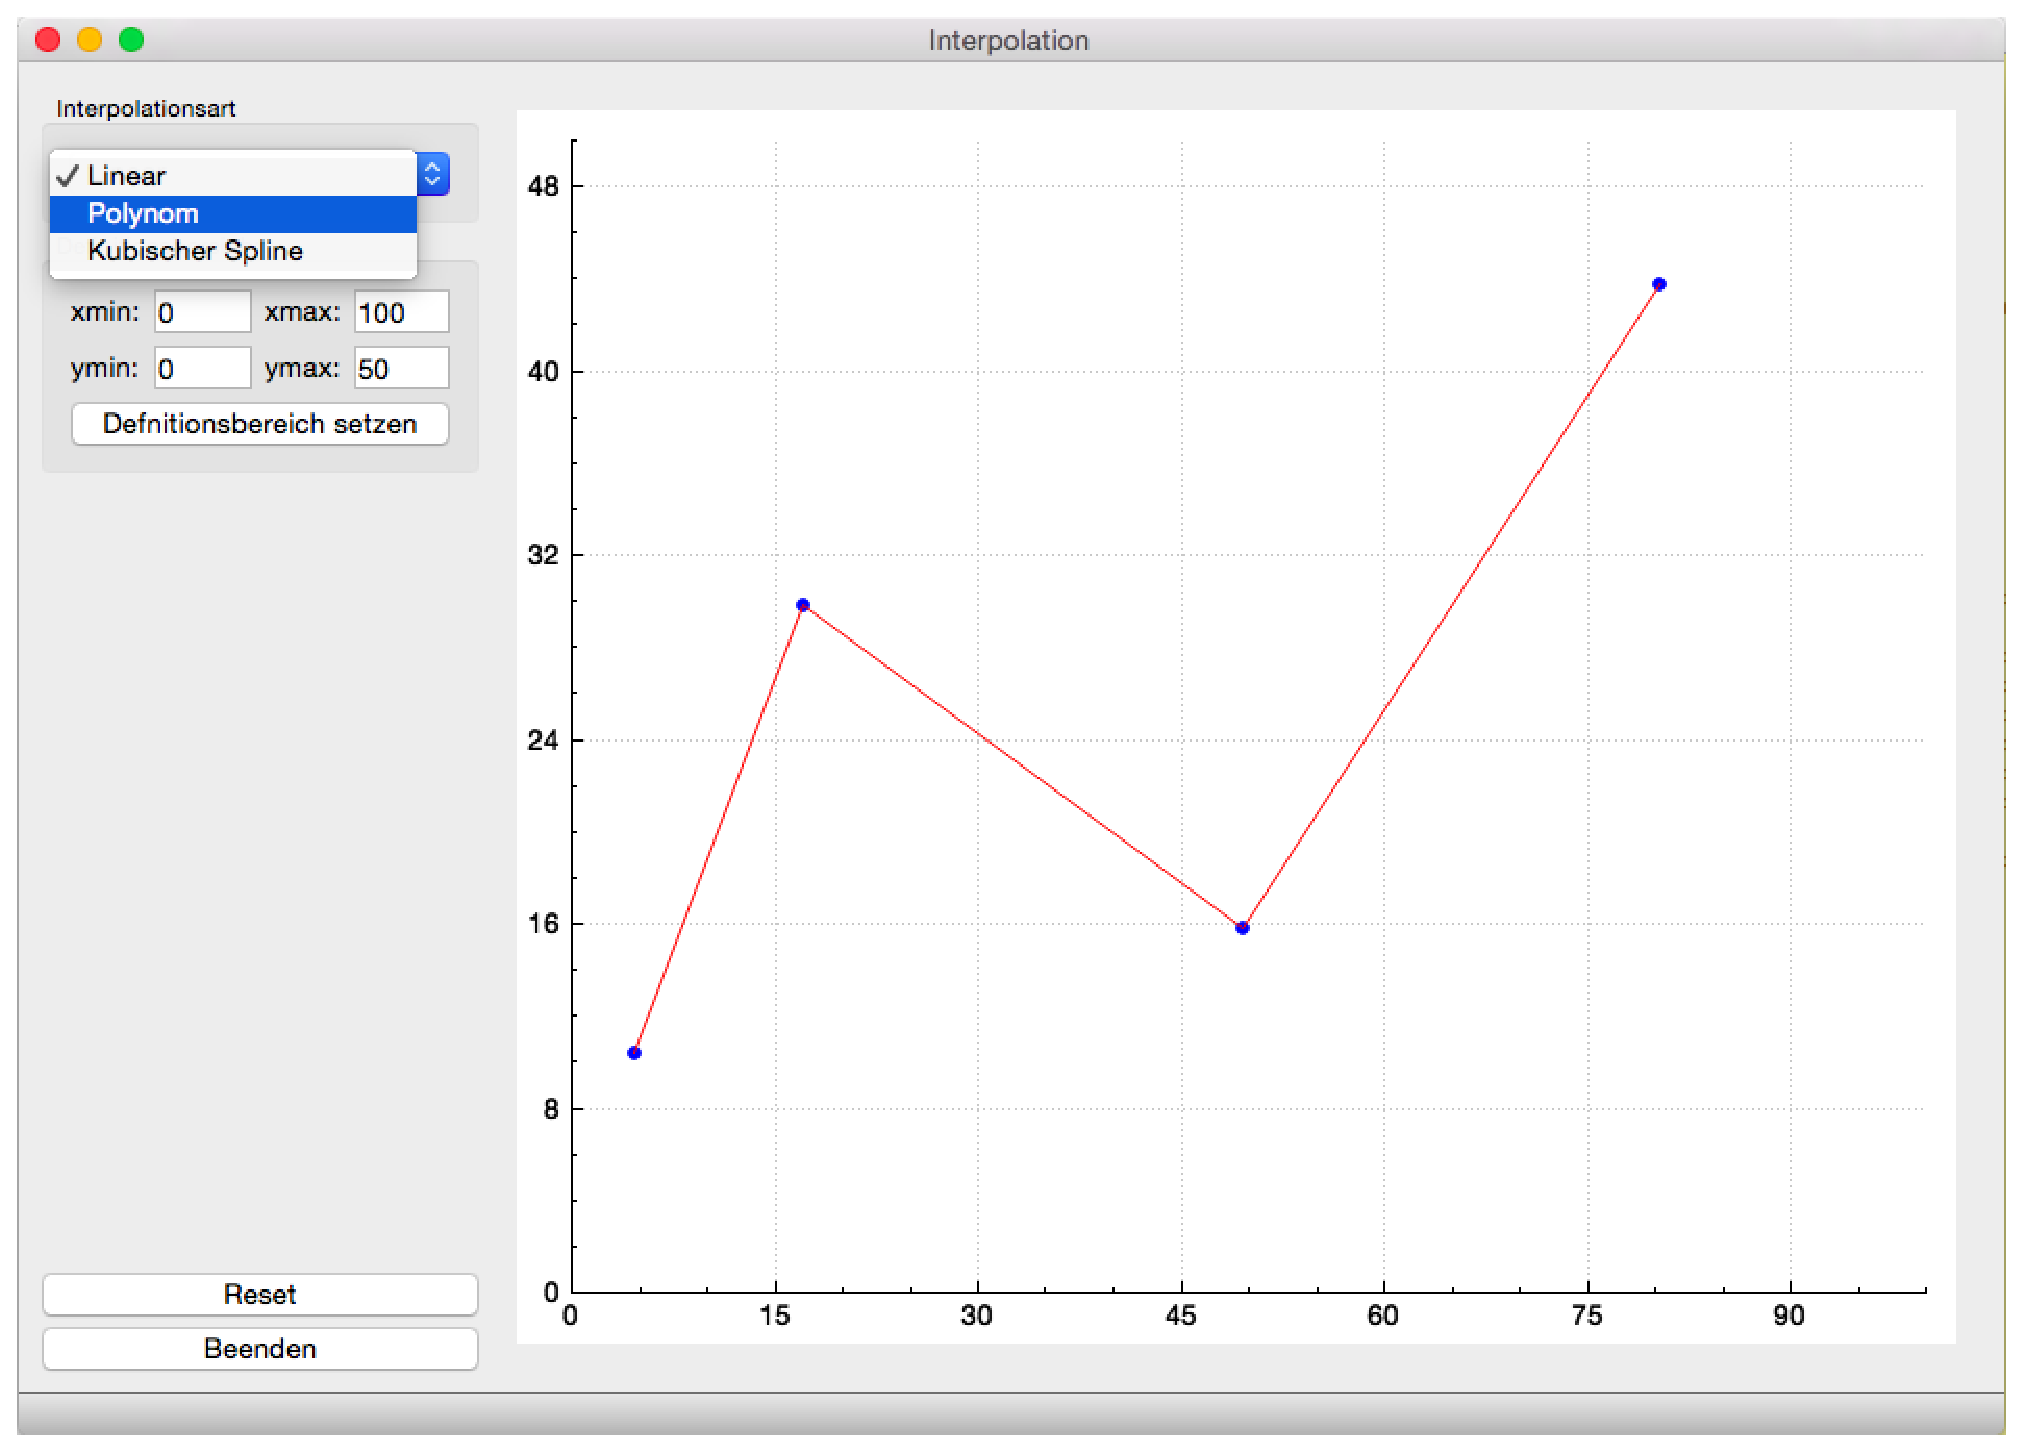
\includegraphics[width=\textwidth]{figures/change_interpol_screen.eps}
\caption{\"Andere Interpolationsart}
\end{figure}

\begin{figure}[H]
\centering
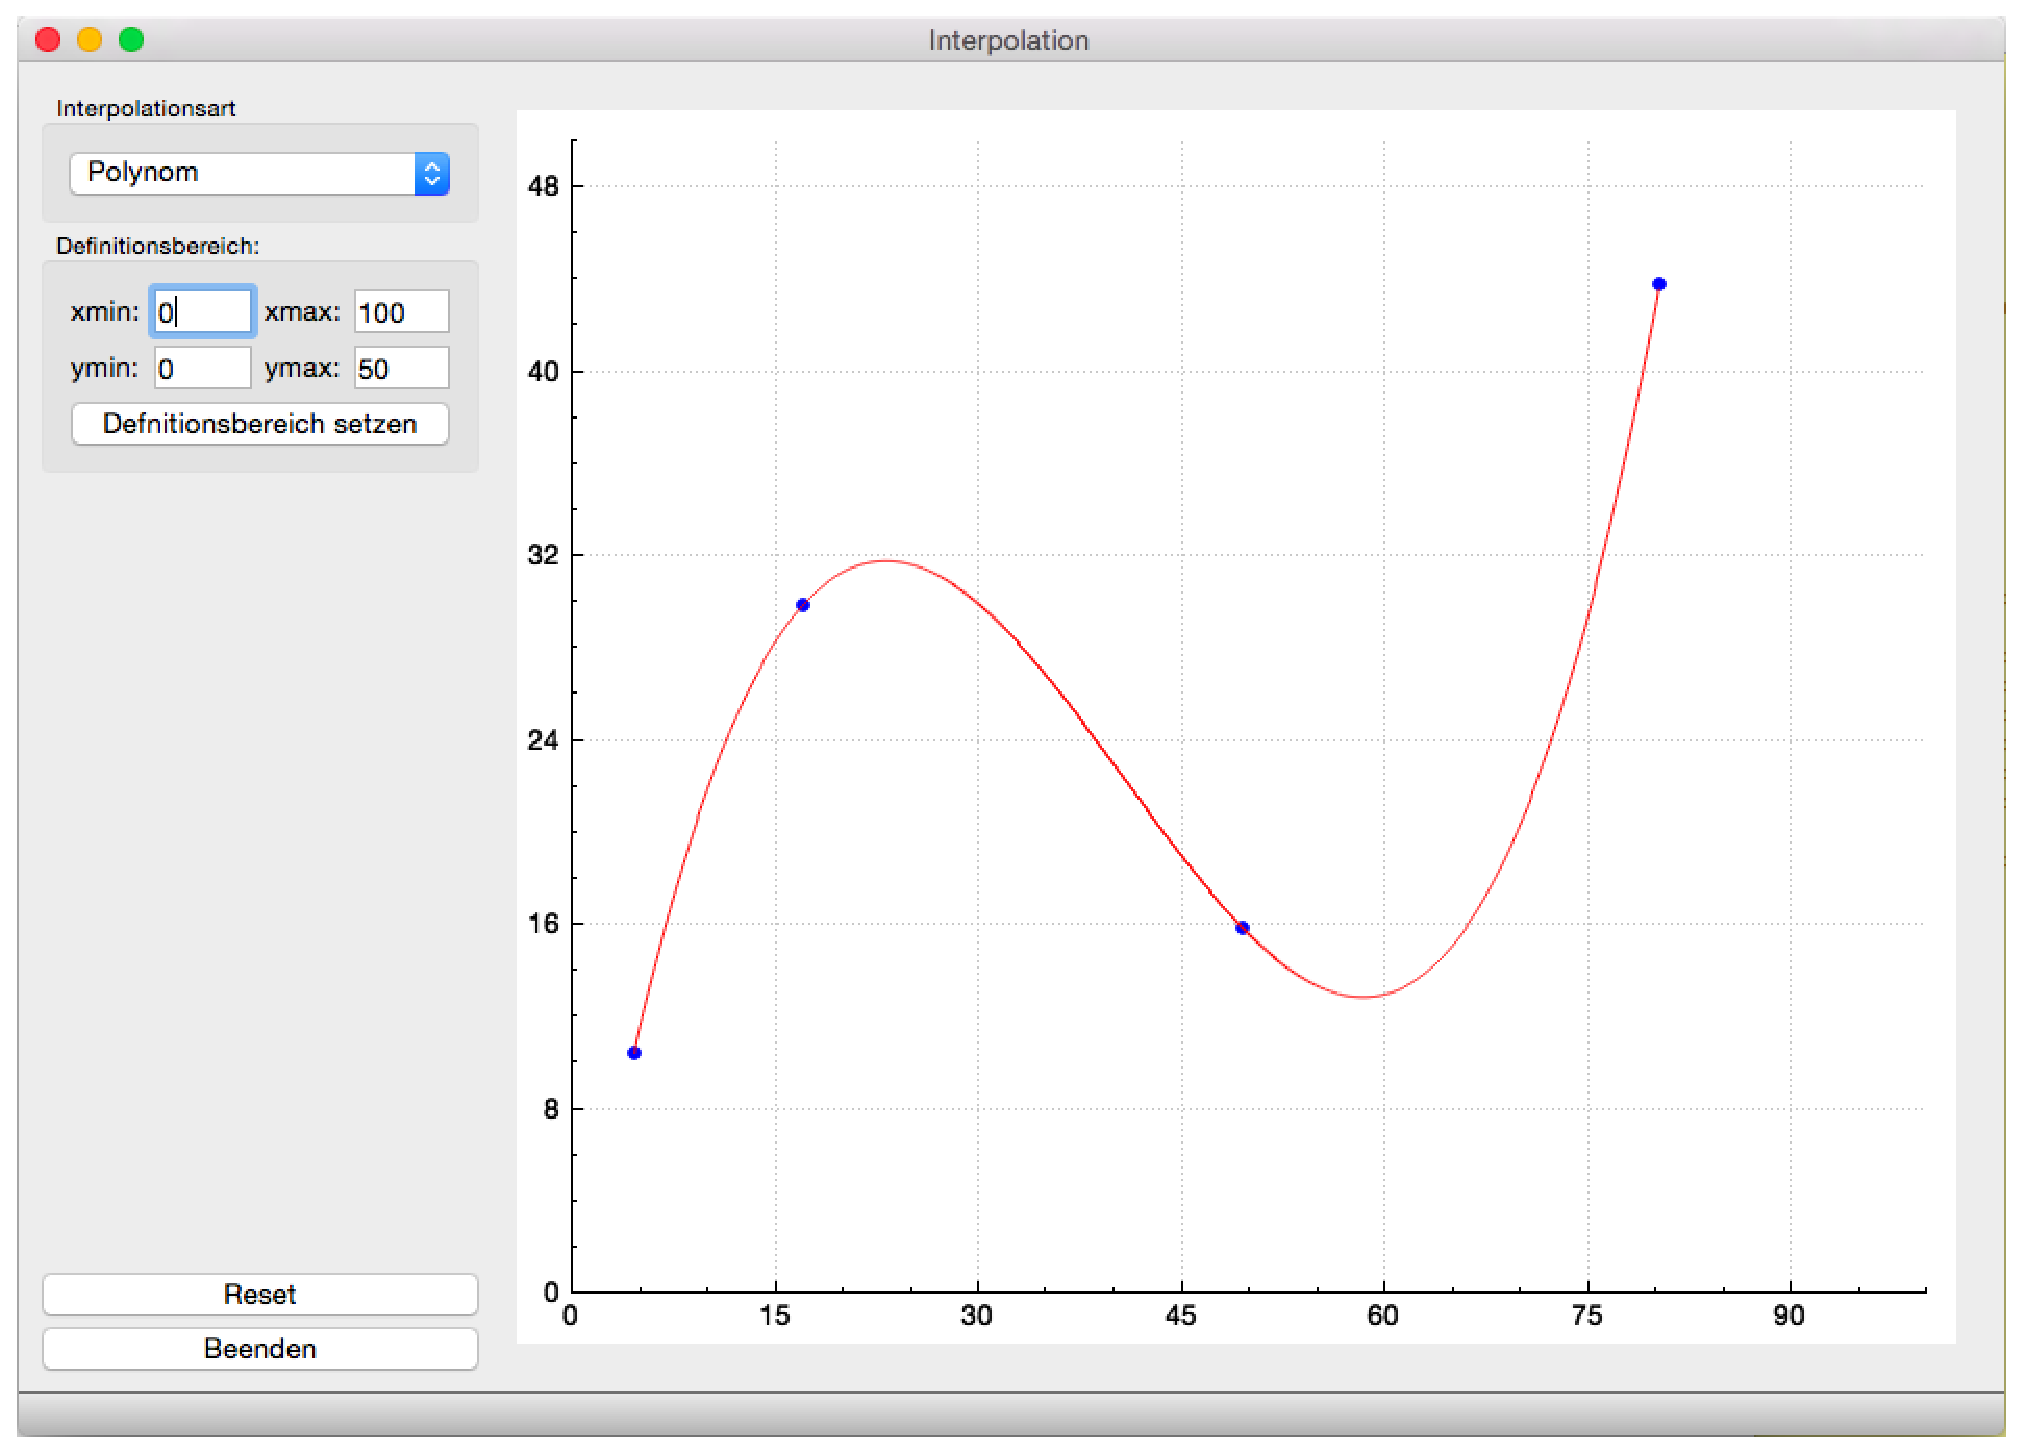
\includegraphics[width=\textwidth]{figures/polynom_interpol_screen.eps}
\caption{Polynominterpolation zwischen Punkten}
\end{figure}

\noindent Der Nutzer ver\"andert den Definitionsbereich durch Eingeben der Grenzen in die entsprechenden Textfelder und Klicken auf die Schaltfl\"ache 'Definitionsbereich setzen' . Sind die Grenzen jedoch nicht konform, d.h. ist xmin z.B. gr\"o\ss er als xmax, so wird eine Fehlermeldung ausgegeben.\\

\begin{figure}[H]
\centering
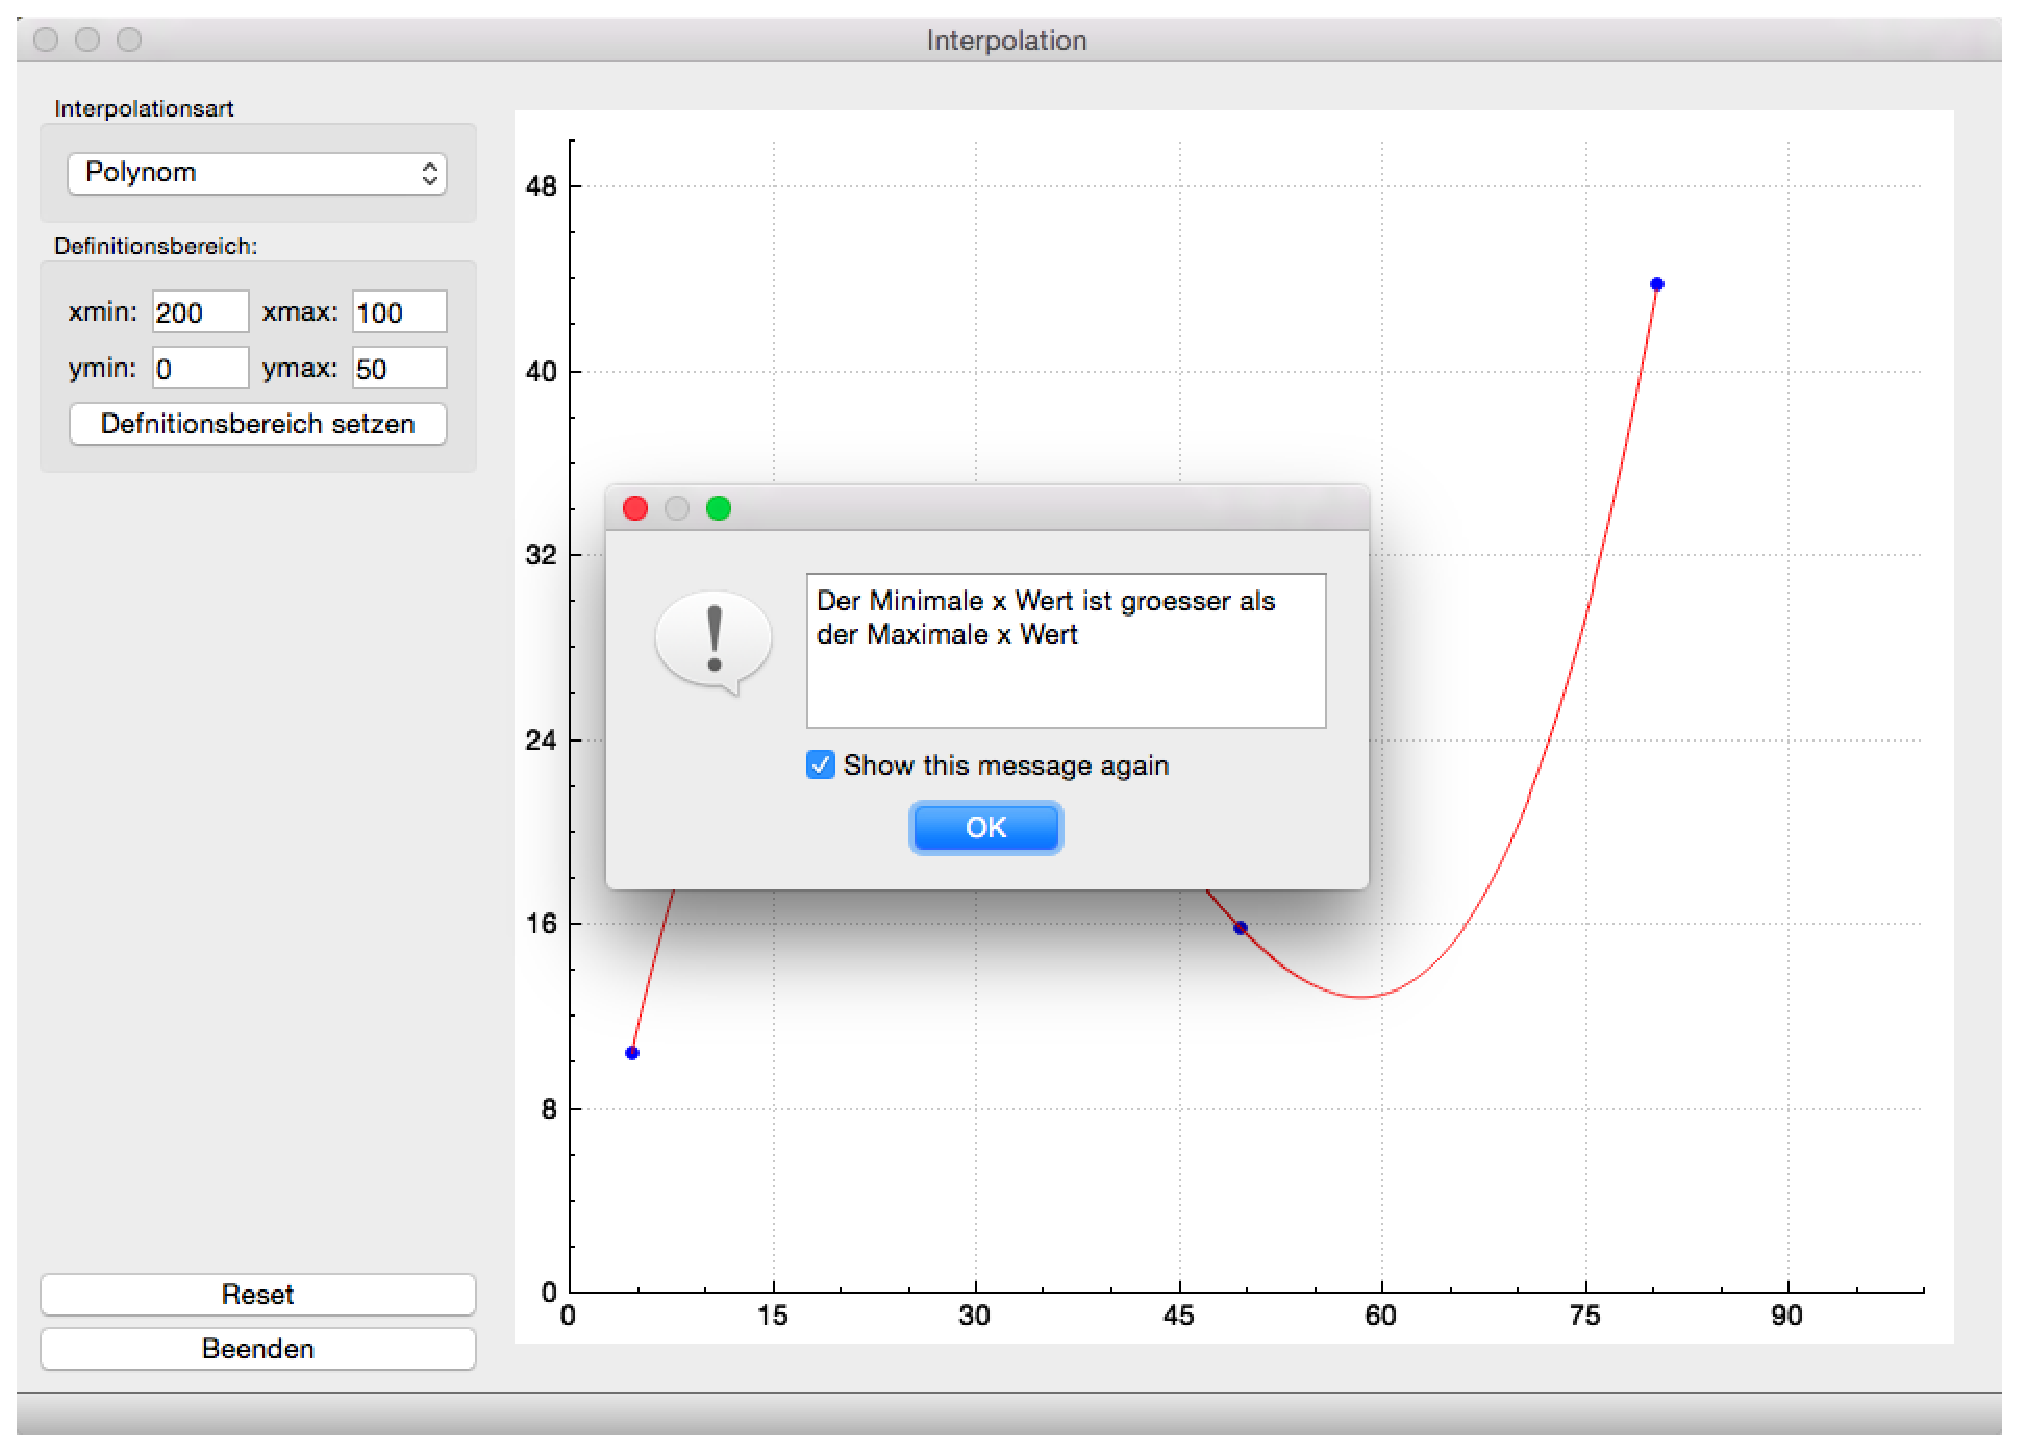
\includegraphics[width=\textwidth]{figures/error_message_screen.eps}
\caption{Anzeige einer Fehlermeldung}
\end{figure}

\noindent Der Nutzer klickt auf die Schaltfl\"ache 'Beenden' und das Programm schlie\ss t. 

\section{Fehlersituationen}
Das Programm gibt Fehlermeldungen aus. Diese k\"onnen nur entstehen, wenn der Definitionsbereich ver\"andert wird. Es wird eine Fehlermeldung ausgegeben, wenn ein Feld leer ist, einen Buchstaben enth\"alt, die Grenzen au\ss erhalb eines vordefinierten Intervalls oder die Anzahl der Nachkommastellen zu gro\ss \ ist. Es sind alle anderen Ausnahmen und m\"ogliche Fehlersituationen so behandelt, dass diese nicht angezeigt werden m\"ussen und sich der Benutzer komplett mit der Bedienung des Programms besch\"aftigen kann. Sollten dennoch Fehler auftreten bitten wir diese an stefan.jeske@rwth-aachen.de zu melden. 






\chapter{Entwicklerdokumentation}
\label{ch:5}

\section{Codestruktur}
Der Code besteht aus mehreren Klassen. Die Quelldateien befinden sich alle im gleichen Verzeichnis. Siehe Kapitel 4 f\"ur Installation. Im Folgenden wird die Codestruktur im Groben beschrieben. F\"ur eine detaillierte Dokumentation siehe Abschnitt 2 in diesem Kapitel.

\subsection{Klasse MainWindow}
Die Klasse {\tt MainWindow} ist f\"ur die graphische Darstellung der Benutzeroberfl\"ache zust\"andig. Der Quellcode findet sich in \refsec{ssec:6.1.1} und in den Dateien {\tt mainwindow.h} und {\tt mainwindow.cpp}.

\subsection{Klasse InterpolationControl}
Die Klasse {\tt InterpolationControl} verwaltet die zur verf\"ugung stehenden Interpolationsarten. Der Quellcode befindet sich in \refsec{ssec:6.1.2} und in den Dateien {\tt interpolationcontrol.h} und {\tt interpolationcontrol.cpp}

\subsection{Klasse Interpolation}
Diese Klasse stellt eine abstrakte Klasse zur Verf\"ugung, welche abgeleitet wird um die einzelnen Interpolationsmethoden zu implementieren. Die Standardm\"a\ss ig verf\"ugbaren Methoden sind lineare Splines, kubische Splines  und Polynominterpolation (Grad m-1, wobei m die Anzahl der St\"utzstellen ist.) Der Quellcode befindet sich jeweils im Anhang \refsec{ssec:6.1.3} und in den Dateien {\tt interpolation.h} und {\tt interpolation.h}.\\ 
Der Quellcode der implementierten Verfahren befindet sich in \refsec{ssec:6.1.4} bis \refsec{ssec:6.1.6}


\section{Detaillierte Dokumentation des Codes}
In dem Unterverzeichnis {\tt ./Interpolation/doc/} befindet sich die Konfigurationsdatei {\tt Doxyfile} f\"ur die Erstellung der doxygen Dokumentation in {\tt HTML} oder \LaTeX\ Format. Zum Erstellen der Dokumentation muss der Befehl {\tt doxygen Doxyfile} in dem Verzeichnis {\tt ./Interpolation/doc/} aufgerufen werden. Es werden zwei neue Verzeichnisse {\tt ./Interpolation/doc/html/} und {\tt ./Interpolation/doc/latex/} erstellt. Um die {\tt HTML} Version anzuzeigen muss in den Ordner {\tt html} gewechselt werden und die Datei {\tt index.html} mit dem Standardbrowser ge\"offnet werden. Um die \LaTeX\ Dokumentation anzeigen zu lassen muss der Befehl {\tt make} in dem Ordner {\tt latex} ausgef\"uhrt werden. Anschlie\ss end kann die PDF Datei mit einem entsprechenden Programm gelesen werden.

\section{Hinzuf\"ugen einer neuen Interpolationsart}
Das Hinzuf\"ugen einer neuen Interpolationsart l\"asst sich in die folgenden Schritte unterteilen. 

\subsection{Ableiten der Klasse Interpolation}
Zun\"achst muss, um eine neue Interpolationsart zu implementieren, die Klasse Interpolation in der folgenden Form abgeleitet werden.

\begin{lstlisting}
#include <interpolation.h>

class myInterpolation : public Interpolation
{
public:
	void StartInterpolation(
            const QVector<double>& xPos,
            const QVector<double>& yPos,
            QVector<double>& xCurve,
            QVector<double>& yCurve
            );
};
\end{lstlisting}

Die eigentliche Interpolation wird durch die Schnittstelle {\tt StartInterpolation(...)} definiert, welche in den Variablen {\tt xCurve, yCurve} die zu {\tt xPos,yPos} geh\"orenden interpolierten Punkte speichert, die zum Zeichnen der Kurve verwendet werden.\\
Diese Methode muss von dem Benutzer in folgender Form implementiert werden:

\begin{lstlisting}

void myInterpolation::StartInterpolation(
            const QVector<double>& xPos,
            const QVector<double>& yPos,
            QVector<double>& xCurve,
            QVector<double>& yCurve
            )
{
	...
	<myImplementation>
	...
}

\end{lstlisting}

\subsection{Hinzuf\"ugen der Interpolationsart in den Quellcode: InterpolationControl}
Angenommen, die neue Interpolationsart wurde in den Dateien {\tt myinterpolation.h} und {\tt myinterpolation.cpp} gespeichert, muss zun\"achst die folgende Zeile zu den {\tt includes} der {\tt interpolationcontrol.h} und ein neues Objekt in den {\tt private:} Teil der Klasse hinzugef\"ugt werden. 

\begin{lstlisting}
...
#include "myinterpolation.h"
...
\end{lstlisting}

\begin{lstlisting}
Interpolation * myInterpolationModel;
\end{lstlisting}

Danach muss in der Datei {\tt interpolationcontrol.cpp} in dem Konstruktor ein Objekt vom Typ {\tt myInterpolation} erzeugt  und in der Funktion {\tt changeActiveModel(...)} ein weiterer switch-case hinzugef\"ugt werden:

\begin{lstlisting} 
InterpolationControl::InterpolationControl()
{
	...
	myInterpolationModel = new myInterpolation();
	...
}

...

void InterpolationControl::changeActiveModel(int _activeModel)
{
	...
	switch(_activeModel)
	{
		...
		case 3 : activeModel = myInterpolationModel;
			str = "myInterpolation ausgewaehlt";
			break;
	}
}
\end{lstlisting}

\subsection{Hinzuf\"ugen der Interpolationsart in den Quellcode: MainWindow}
Zuletzt muss noch eine Zeile am Ende des Konstruktors der Klasse {\tt MainWindow} eingef\"ugt werden.
\begin{lstlisting}
MainWindow::MainWindow(QWidget *parent) :
    QMainWindow(parent),
    ui(new Ui::MainWindow)
{
	...
	ui->interpolation_select->addItem("myInterpolation");
}
\end{lstlisting}
Nun befindet sich ein weiterer Eintrag {\tt myInterpolation} in der Auswahlbox auf der Benutzeroberfl\"ache und kann ausgew\"ahlt werden, um die Punkte auf der Zeichenfl\"ache mit {\tt myInterpolation} zu verbinden.

\section{Software-Tests}
Alle Anwendungsf\"alle wurden manuell auf Funktionalit\"at getestet. Die folgenden Anwendungsf\"alle wurden erfolgreich ohne Fehlermeldungen getestet:
\begin{itemize}
  \item Interpolationsart \"andern
  \item Reset
  \item Beenden
  \item St\"utzstelle l\"oschen
  \item St\"utzstelle hinzuf\"ugen
\end{itemize}
Der Anwendungsfall 'Definitionsbereich \"andern' wurde erfolgreich mit allen Fehlersituationen getestet, die in der Benutzerdokumentation ausf\"uhrlich beschrieben sind.










\bibliographystyle{plain}
\bibliography{analyse_entwurf}

\appendix

\chapter{Quellcode}
\label{ch:6}

\section{Interpolation}
\label{sec:6.1}

\subsection{Klasse MainWindow}
\label{ssec:6.1.1}

\lstinputlisting[caption={mainwindow.h}]{../Projekt/Interpolation/mainwindow.h}
\lstinputlisting[caption={mainwindow.cpp}]{../Projekt/Interpolation/mainwindow.cpp}

\subsection{Klasse InterpolationControl}
\label{ssec:6.1.2}

\lstinputlisting[caption={interpolationcontrol.h}]{../Projekt/Interpolation/interpolationcontrol.h}
\lstinputlisting[caption={interpolationcontrol.cpp}]{../Projekt/Interpolation/interpolationcontrol.cpp}

\subsection{Klasse Interpolation}
\label{ssec:6.1.3}

\lstinputlisting[caption={interpolation.h}]{../Projekt/Interpolation/interpolation.h}
\lstinputlisting[caption={interpolation.cpp}]{../Projekt/Interpolation/interpolation.cpp}

\subsection{Klasse CubicSpline}
\label{ssec:6.1.4}

\lstinputlisting[caption={cubicspline.h}]{../Projekt/Interpolation/cubicspline.h}
\lstinputlisting[caption={cubicspline.cpp}]{../Projekt/Interpolation/cubicspline.cpp}

\subsection{Klasse PolynomialInterpolation}
\label{ssec:6.1.5}

\lstinputlisting[caption={polynomialinterpolation.h}]{../Projekt/Interpolation/polynomialinterpolation.h}
\lstinputlisting[caption={polynomialinterpolation.cpp}]{../Projekt/Interpolation/polynomialinterpolation.cpp}

\subsection{Klasse LinearSpline}
\label{ssec:6.1.6}

\lstinputlisting[caption={linearspline.h}]{../Projekt/Interpolation/linearspline.h}
\lstinputlisting[caption={linearspline.cpp}]{../Projekt/Interpolation/linearspline.cpp}

\subsection{Main Datei}
\label{ssec:6.1.7}

\lstinputlisting[caption={main.cpp}]{../Projekt/Interpolation/main.cpp}


\end{document}

